\documentclass[letterpaper]{article} 
\usepackage[utf8]{inputenc}
\usepackage[T1]{fontenc}
\usepackage{amsmath}
\usepackage{amsfonts}
\usepackage{amssymb}
\usepackage{hyperref}
\usepackage[version=4]{mhchem}
\usepackage{stmaryrd}
\usepackage[dvipsnames]{xcolor}
\colorlet{LightRubineRed}{RubineRed!70}
\colorlet{Mycolor1}{green!10!orange}
\definecolor{Mycolor2}{HTML}{00F9DE}
\usepackage{graphicx}
\usepackage{amsmath}
\usepackage{graphicx}
\usepackage{capt-of}
\usepackage{lipsum}
\usepackage{fancyvrb}
\usepackage{tabularx}
\usepackage{listings}
\usepackage[export]{adjustbox}
\graphicspath{ {./images/} }
\usepackage[utf8]{inputenc}
\usepackage[english]{babel}
\usepackage{float}
\usepackage{lipsum}
\usepackage{graphicx}
\usepackage{float}
\usepackage[margin=0.7in]{geometry}
\usepackage{amsmath}
\usepackage{graphicx}
\usepackage{capt-of}
\usepackage{tcolorbox}
\usepackage{lipsum}
\usepackage{graphicx}
\usepackage{float}
\usepackage{listings}
\usepackage{hyperref} 
\usepackage{xcolor} % For custom colors
\lstset{
	language=Python,                % Choose the language (e.g., Python, C, R)
	basicstyle=\ttfamily\small, % Font size and type
	keywordstyle=\color{blue},  % Keywords color
	commentstyle=\color{gray},  % Comments color
	stringstyle=\color{red},    % String color
	numbers=left,               % Line numbers
	numberstyle=\tiny\color{gray}, % Line number style
	stepnumber=1,               % Numbering step
	breaklines=true,            % Auto line break
	backgroundcolor=\color{black!5}, % Light gray background
	frame=single,               % Frame around the code
}
\usepackage{float}
\usepackage[]{amsthm} %lets us use \begin{proof}
\usepackage[]{amssymb} %gives us the character \varnothing


	\title{Homework 2, MATH 5010}
	\author{Zongyi Liu}
	\date{Feb 28, 2025}
	\begin{document}
		\maketitle
		
		\subsubsection*{Question 1}
		What is the difference between historic and implied volatilities? Which one is higher for Microsoft stock MSFT? Go to the Bloomberg terminal and type: \texttt{MSFT <Equity> HIVG <Go>}. Print the output.
		
		\textbf{Answer}
		
		 
		 The Historical Volatility is also called \underline{Realized Volatility} or \underline{Statistical Volatility}, and it measures the actual volatility of an asset's price over a specific past period. It is calculated using historical price data (e.g., daily, weekly, or monthly returns).
				
				Historic Volatility is typically calculated as the \underline{standard deviation} of the asset's logarithmic returns over a given time frame. The formula is:
				\[
				\text{Historic Volatility} = \sqrt{\frac{1}{N-1} \sum_{i=1}^{N} (r_i - \bar{r})^2}
				\]
				where:
				\begin{itemize}
					\item \( r_i \): logarithmic return at time \( i \),
					\item \( \bar{r} \): average return over the period,
					\item \( N \): number of observations.
				\end{itemize}
				
			
			As for the Implied Volatility (IV), it is a forward-looking measure of volatility derived from the market price of an option. It represents the market's expectation of future volatility over the option's life.
				
			
			Implied Volatility is not directly calculated but is inferred using an options pricing model (e.g. the Black-Scholes model). It is the value of volatility that, when plugged into the model, matches the market price of the option. The Black-Scholes formula for a call option is:
				\[
				C = S_0 N(d_1) - K e^{-rT} N(d_2)
				\]
				where:
				
				\begin{itemize}
					\item \( C \): market price of the call option,
					\item \( S_0 \): current price of the underlying asset,
					\item \( K \): strike price,
					\item \( r \): risk-free rate,
					\item \( T \): time to expiration,
					\item \( N(d) \): cumulative distribution function of the standard normal distribution,
					\item \( d_1 \) and \( d_2 \): functions of volatility (\( \sigma \)).
				\end{itemize}
				Implied Volatility is the value of \( \sigma \) that satisfies this equation.
				
				Finally, for their relationship, over time, implied volatility tends to converge toward historic volatility as the future becomes the past. Implied volatility can be higher or lower than historic volatility depending on market expectations (e.g., during periods of uncertainty or calm).
				
				We can use a table to illustrate this:
			
			\begin{center}
				\resizebox{\linewidth}{!}{
				\begin{tabular}{|l|l|l|}
					\hline
					\textbf{Aspect} & \textbf{Historic Volatility} & \textbf{Implied Volatility} \\
					\hline
					\textbf{Time Frame} & Based on past price movements. & Based on future expectations. \\
					\hline
					\textbf{Data Used} & Historical price data. & Market price of options. \\
					\hline
					\textbf{Calculation} & Calculated using statistical methods (e.g., standard deviation). & Derived from options pricing models (e.g., Black-Scholes). \\
					\hline
					\textbf{Purpose} & Measures past price fluctuations. & Predicts future price fluctuations. \\
					\hline
					\textbf{Market Sentiment} & Does not reflect market sentiment. & Reflects market sentiment and expectations. \\
					\hline
					\textbf{Use in Trading} & Used for risk analysis and benchmarking. & Used for options pricing and trading strategies. \\
					\hline
				\end{tabular}
			}
			\end{center}
			
		
		Here is the plot provided by Bloomberg Terminal, and the timespan I set was Sept 16, 2020 to Feb 20, 2025.
		
		\begin{figure}[h]
			\caption{The Results after using \texttt{MSFT <Enquity> HIVG <GO>}}
			\centering
			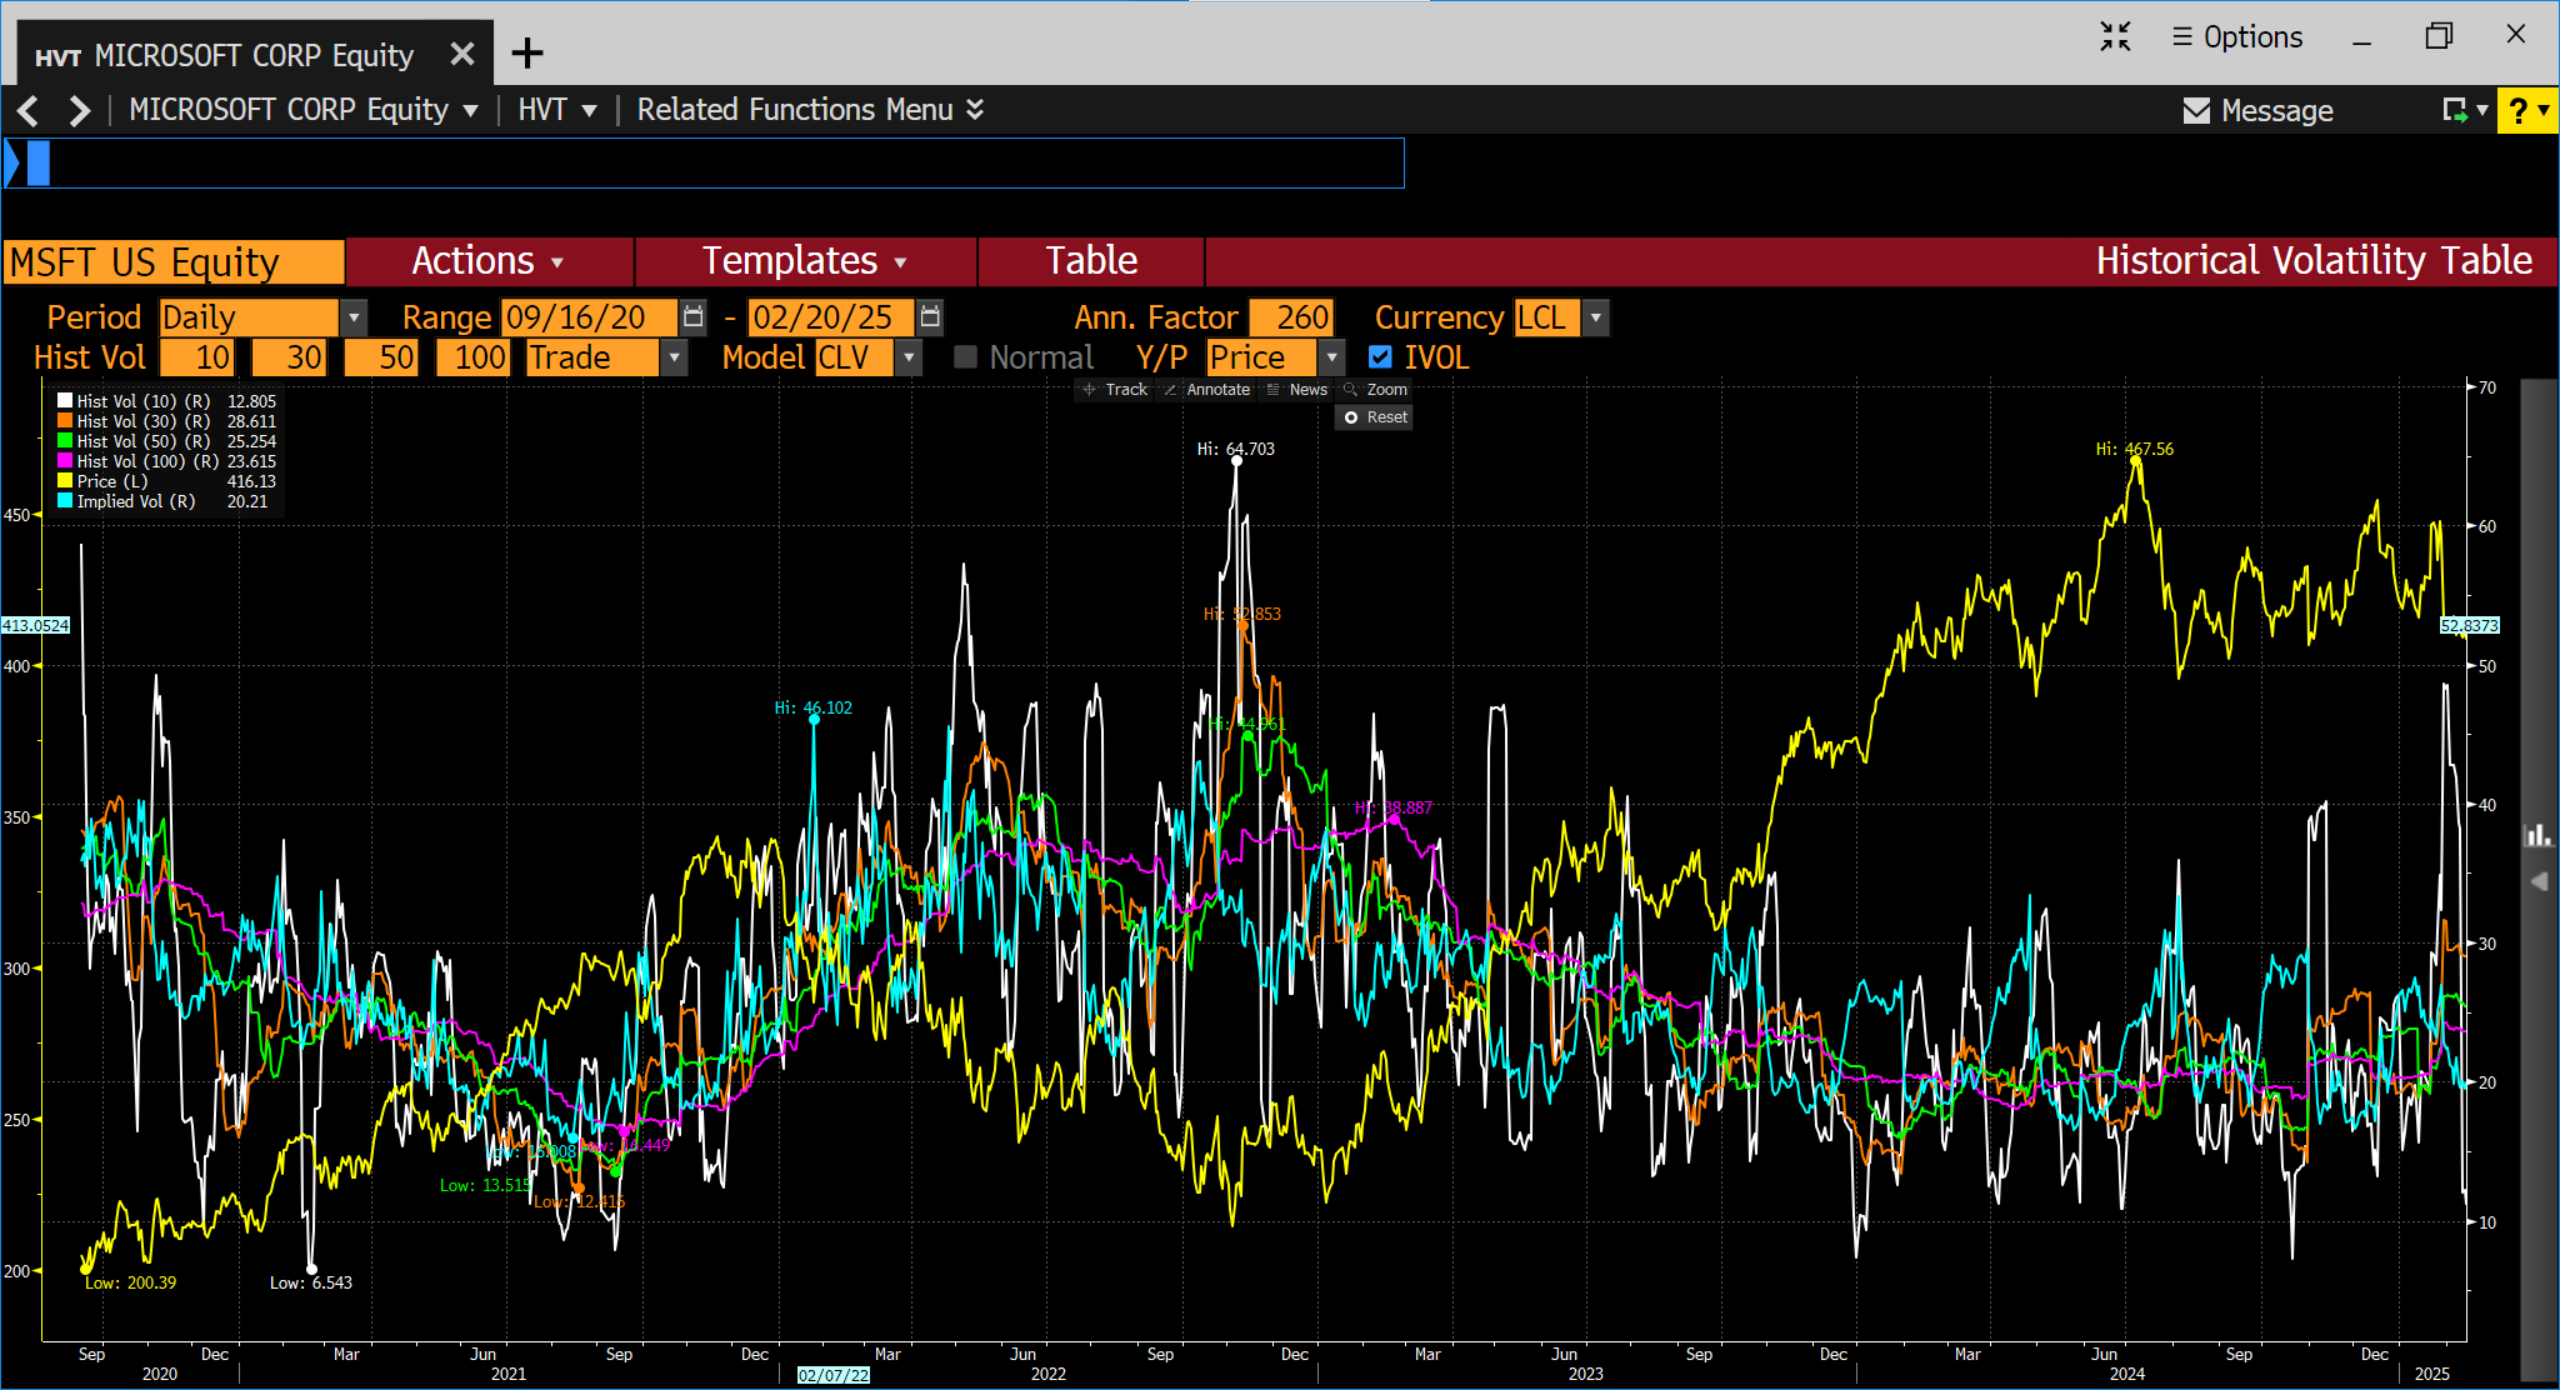
\includegraphics[width=0.8\textwidth]{Q1_1}
		\end{figure}
	
	  Take the date Feb 28, 2025 as the last date for consideration, for a 30-days range, the historical volatility (HV) is 25.99\%, which is higher than the implied volatility (IV), which was around 24.51\%. The exact data can be found \href{https://www.alphaquery.com/stock/MSFT/volatility-option-statistics/30-day/historical-volatility}{here}.
	  
	  However, if we reconsider it in a large time span, the overall Historical Volatility is smaller than the Implied Volatility. It can be easily seen from the graph, and we can also scrutinize the  \href{https://www.alphaquery.com/stock/MSFT/volatility-option-statistics/180-day/historical-volatility}{180-day-data}.
	  
		
			\begin{figure}
				\caption{A Simple Plot Showing HV and IV of MSFT}
			\centering
			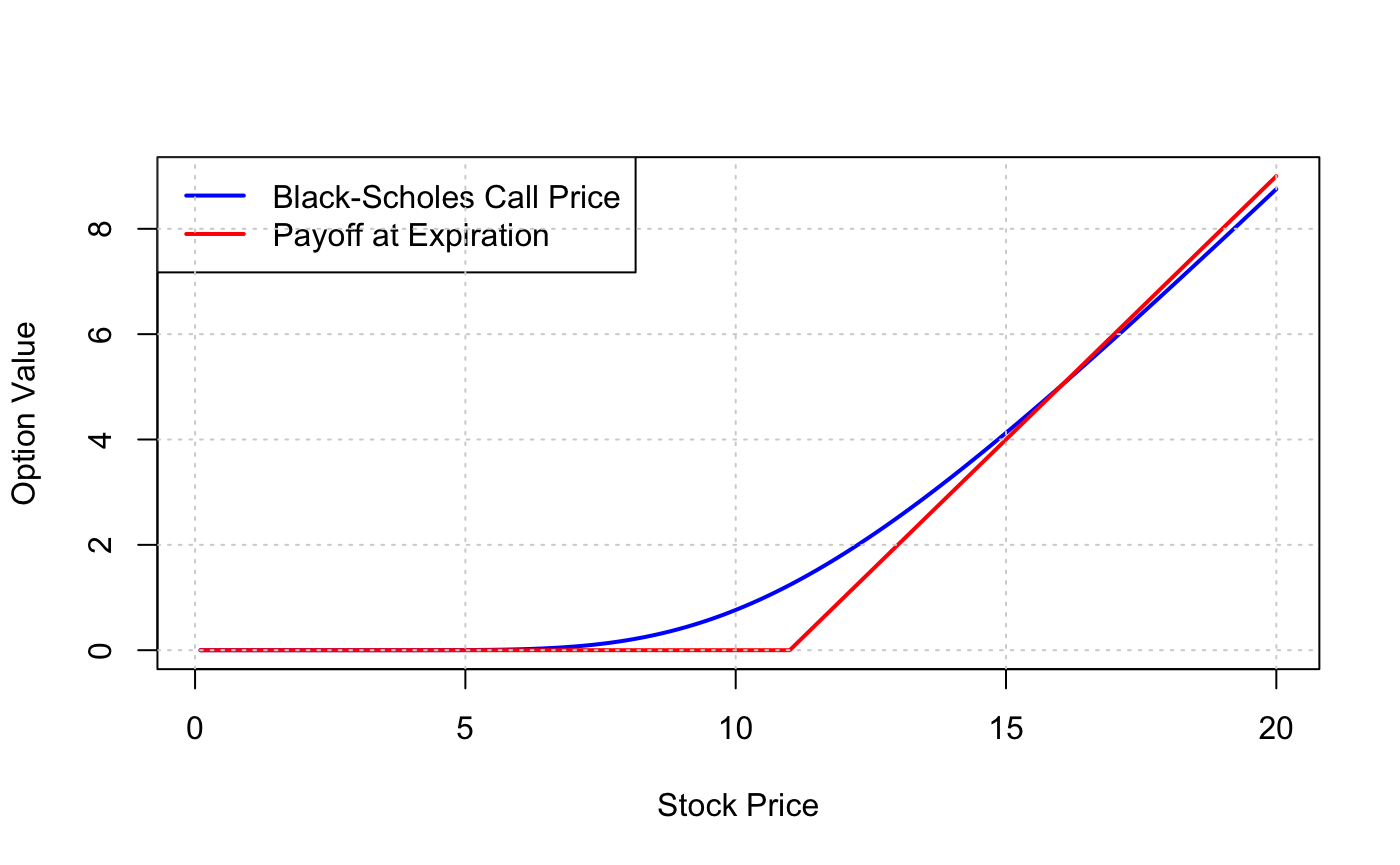
\includegraphics[width=0.8\textwidth]{Q1_2}
		\end{figure}
	
		\clearpage
		
		\subsubsection*{Question 2}
		What is the volatility smile? Using Bloomberg terminal function SKEW (\texttt{CLJ5 Comdty SKEW <Go>}) plot the implied volatility smiles for \texttt{TYH5 Comdty, CLJ5 Comdty, NGJ25 Comdty, ESH5 Index, SPY Equity}. What are these securities? For description type \texttt{CLJ5 Comdty DES}. Compare their smiles. Submit printouts. 
		
		
		\textbf{Answer}
		
		In the Textbook, the author defines Volatility Smile as "A plot of the implied volatility of an option with a certain life as a function of its strike price." (Hull, 409)
		
		In my understanding, Volatility Smile is a pattern observed in the implied volatility of options across different strike prices, where implied volatility is higher for both out-of-the-money (OTM) puts and calls compared to at-the-money (ATM) options, creating a "smile" shape when plotted. This phenomenon contradicts the assumption of constant volatility in models like Black-Scholes and arises because markets often price in higher uncertainty for extreme price movements (both up and down). 
		
		The x-axis is Strike Price, whereas the y-axis is Implied Volatility.
		
		\begin{figure}[h]
			\caption{Simple Illustration of VS (\href{https://www.sciencedirect.com/science/article/pii/S0140988319302324}{cred to Soini et al.})}
			\centering
			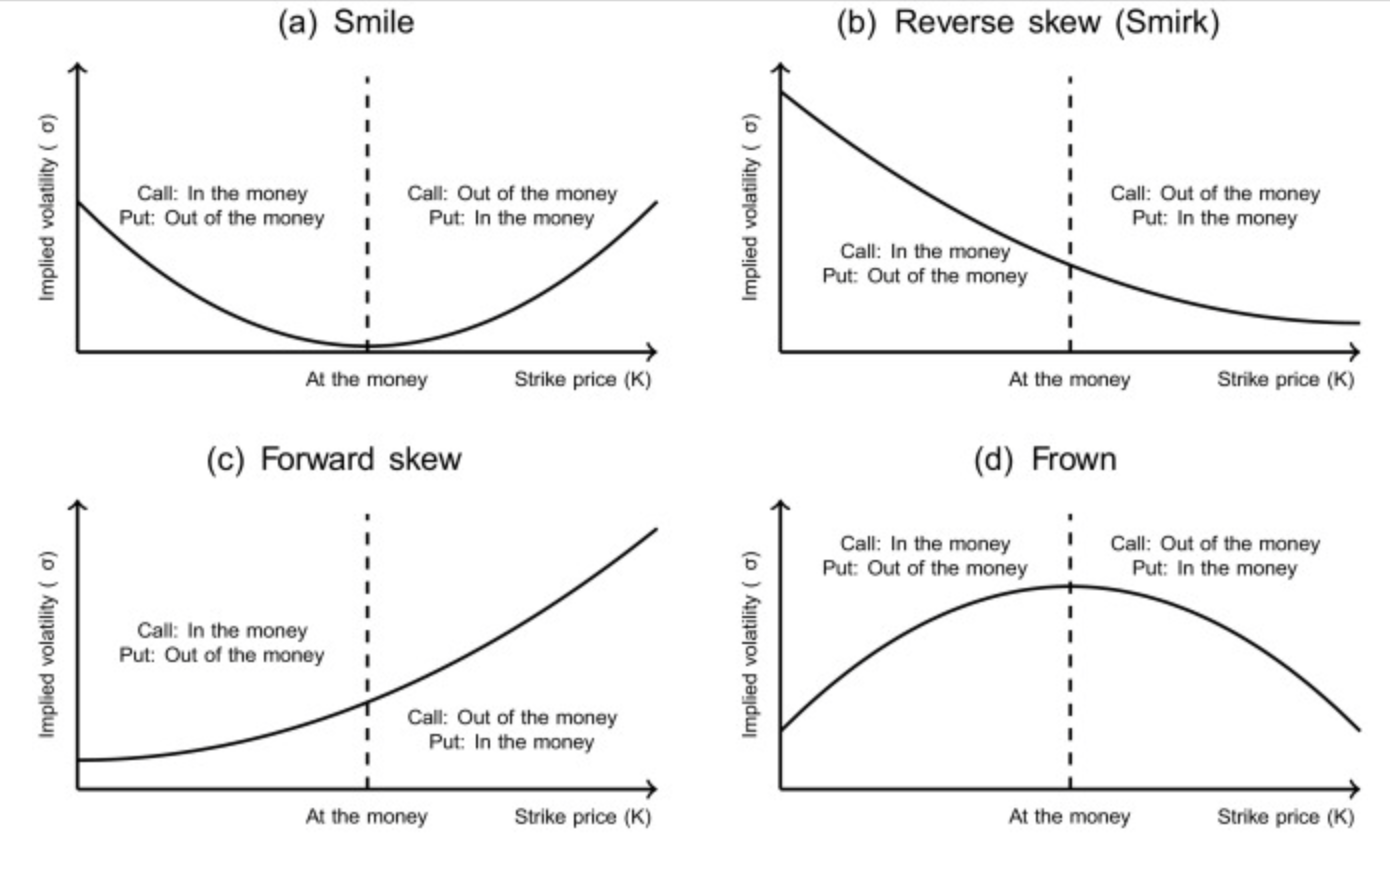
\includegraphics[width=0.7\textwidth]{Q2_0}
		\end{figure}
	
		In Bloomberg, they represent:
		
		\begin{itemize}
			\item \texttt{TYH5 Comdty}: U.S. 10-Year Treasury Futures Contract (April 2025).
			\item \texttt{CLJ5 Comdty}: Crude Oil Futures (April 2025).
			\item \texttt{NGJ25 Comdty}: Natural Gas Futures (April 2025).
			\item \texttt{ESH5 Index}: S\&P 500 E-mini Futures (March 2025).
			\item \texttt{SPY Equity}: SPDR S\&P 500 ETF Trust.
		\end{itemize}

		Here is the graph of volatility smile in Bloomberg Terminal. The model I set was \texttt{Strike} instead of \texttt{Delta} or so, because in \texttt{Delta} mode, there are only four comparable niches, and it is more standard to show their volatility smiles with strike price; moreover, the overall trend will not be impacted by different x-axises we chose.
		
		Take \texttt{Strike} as the x-axis, the Volatility Surface has a Smirk Shape, or Reverse Skew for \texttt{CLJ5 Comdty}, and it reflects a market expectation of greater downside risk than upside potential. It is characterized by higher implied volatility for OTM puts compared to OTM calls and is often driven by bearish sentiment, economic uncertainty, or fear of sharp declines. In such scenarios, OTM puts become more expensive due to higher implied volatility, while OTM calls are relatively cheaper. Traders may use strategies like put spreads or risk reversals to capitalize on this skew, while investors might hedge against potential price declines. 
		
		\begin{figure}
			\caption{Volatility Surface of \texttt{CLJ5 Comdty}}
			\centering
			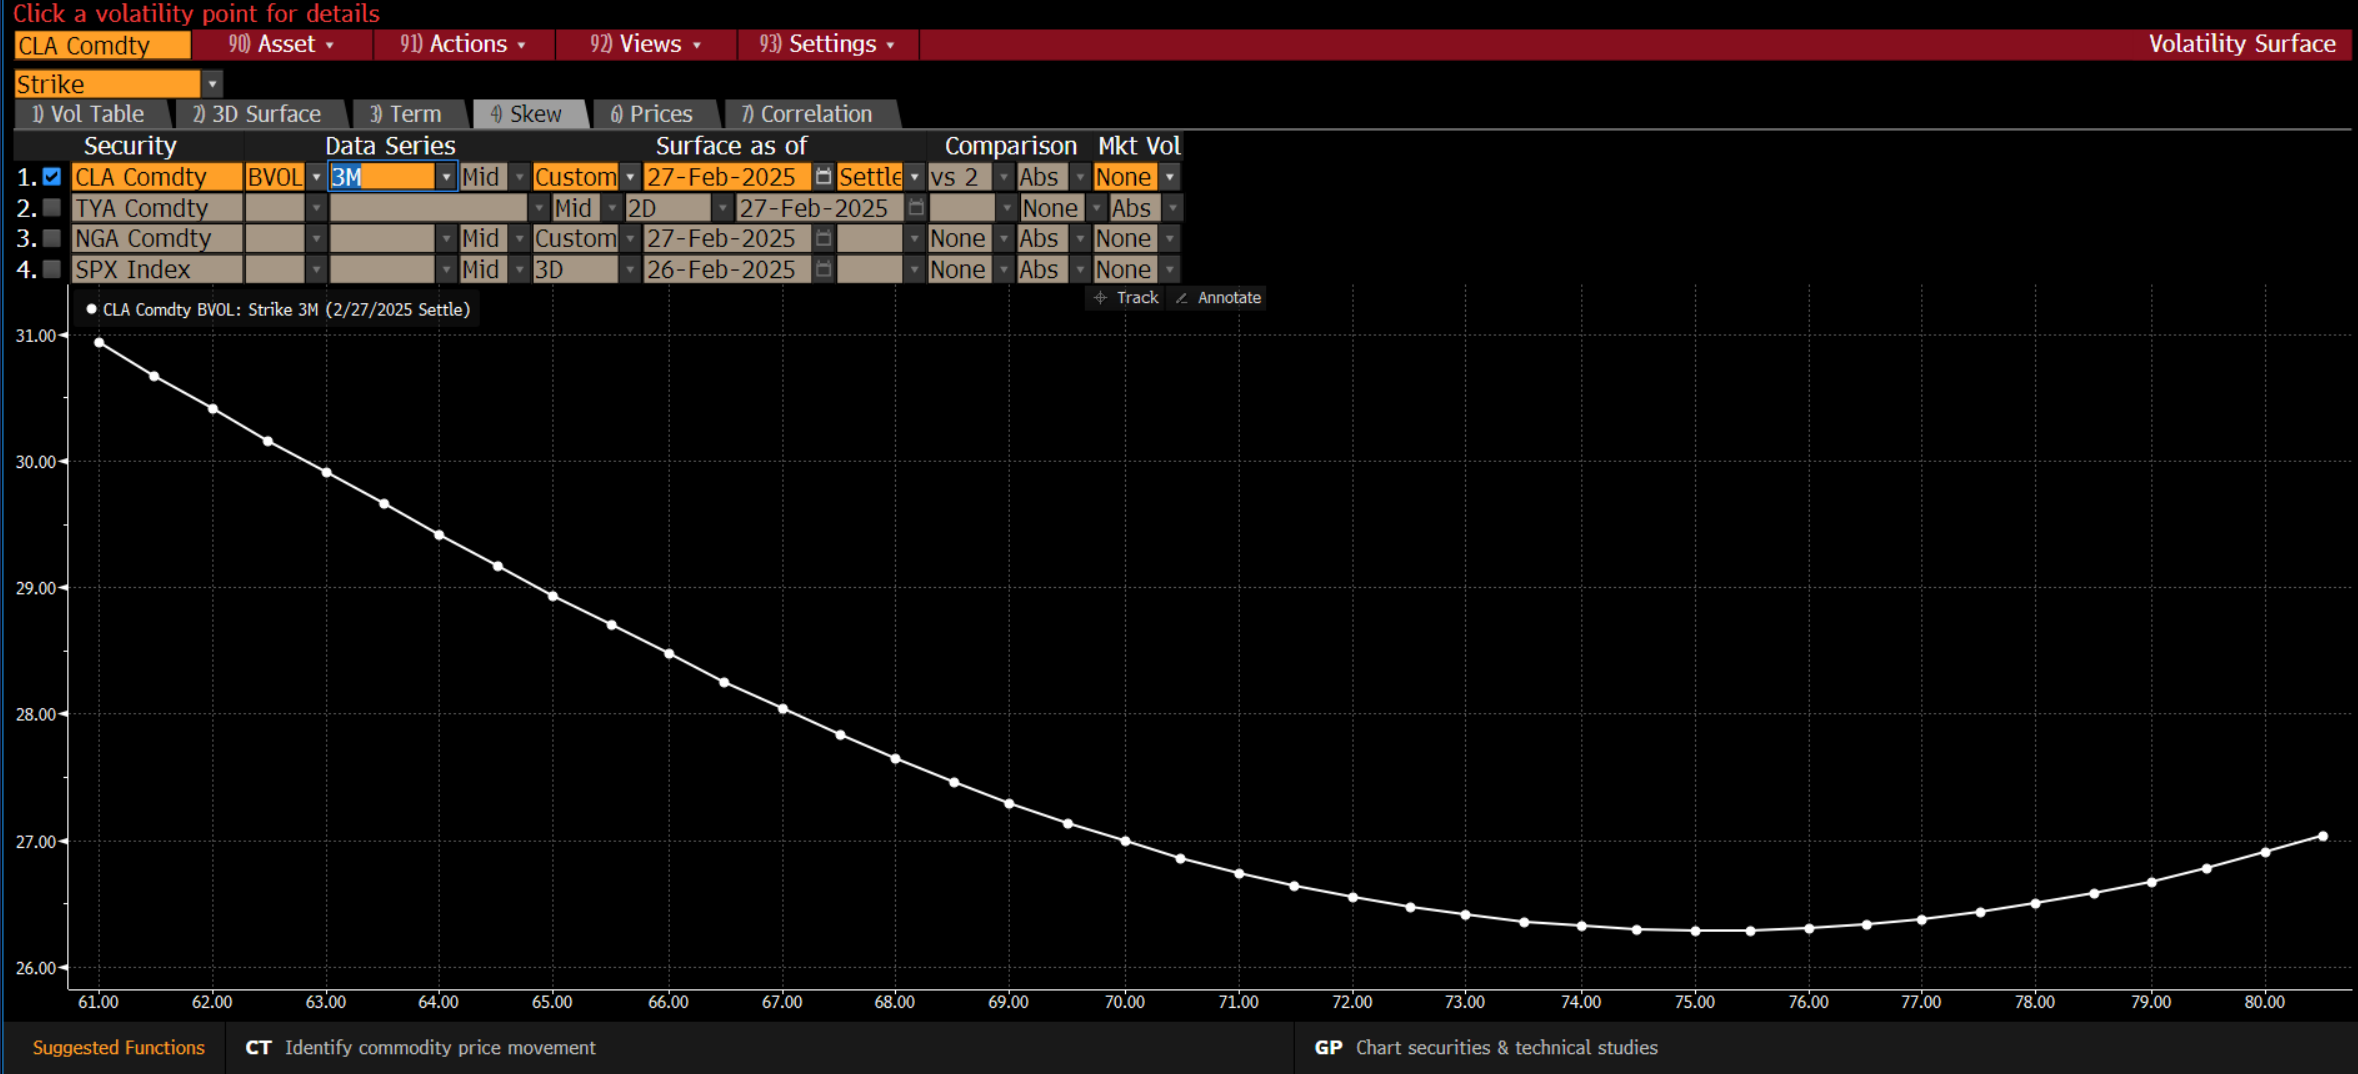
\includegraphics[width=1\textwidth]{Q2_1}
		\end{figure}
	
	For both \texttt{TYH5 Comdty} and \texttt{NGJ5 Comdty}, we have a shape as Forward Skew, meaning its implied volatility is higher for out-of-the-money (OTM) calls (higher strike prices) compared to out-of-the-money (OTM) puts (lower strike prices). This creates an upward-sloping asymmetry in the volatility curve. This pattern indicates that the market expects greater upside potential (price increases) than downside risk (price decreases), often driven by bullish sentiment, anticipated positive events (e.g., earnings reports, supply constraints), or speculative demand. In such scenarios, OTM calls become more expensive due to higher implied volatility, while OTM puts are relatively cheaper. Traders may use strategies like call spreads or risk reversals to capitalize on this skew, while investors might hedge against potential price increases. 
	
	\begin{figure}[h]
			\caption{Volatility Surface of \texttt{TYH5 Comdty}}
		\centering
		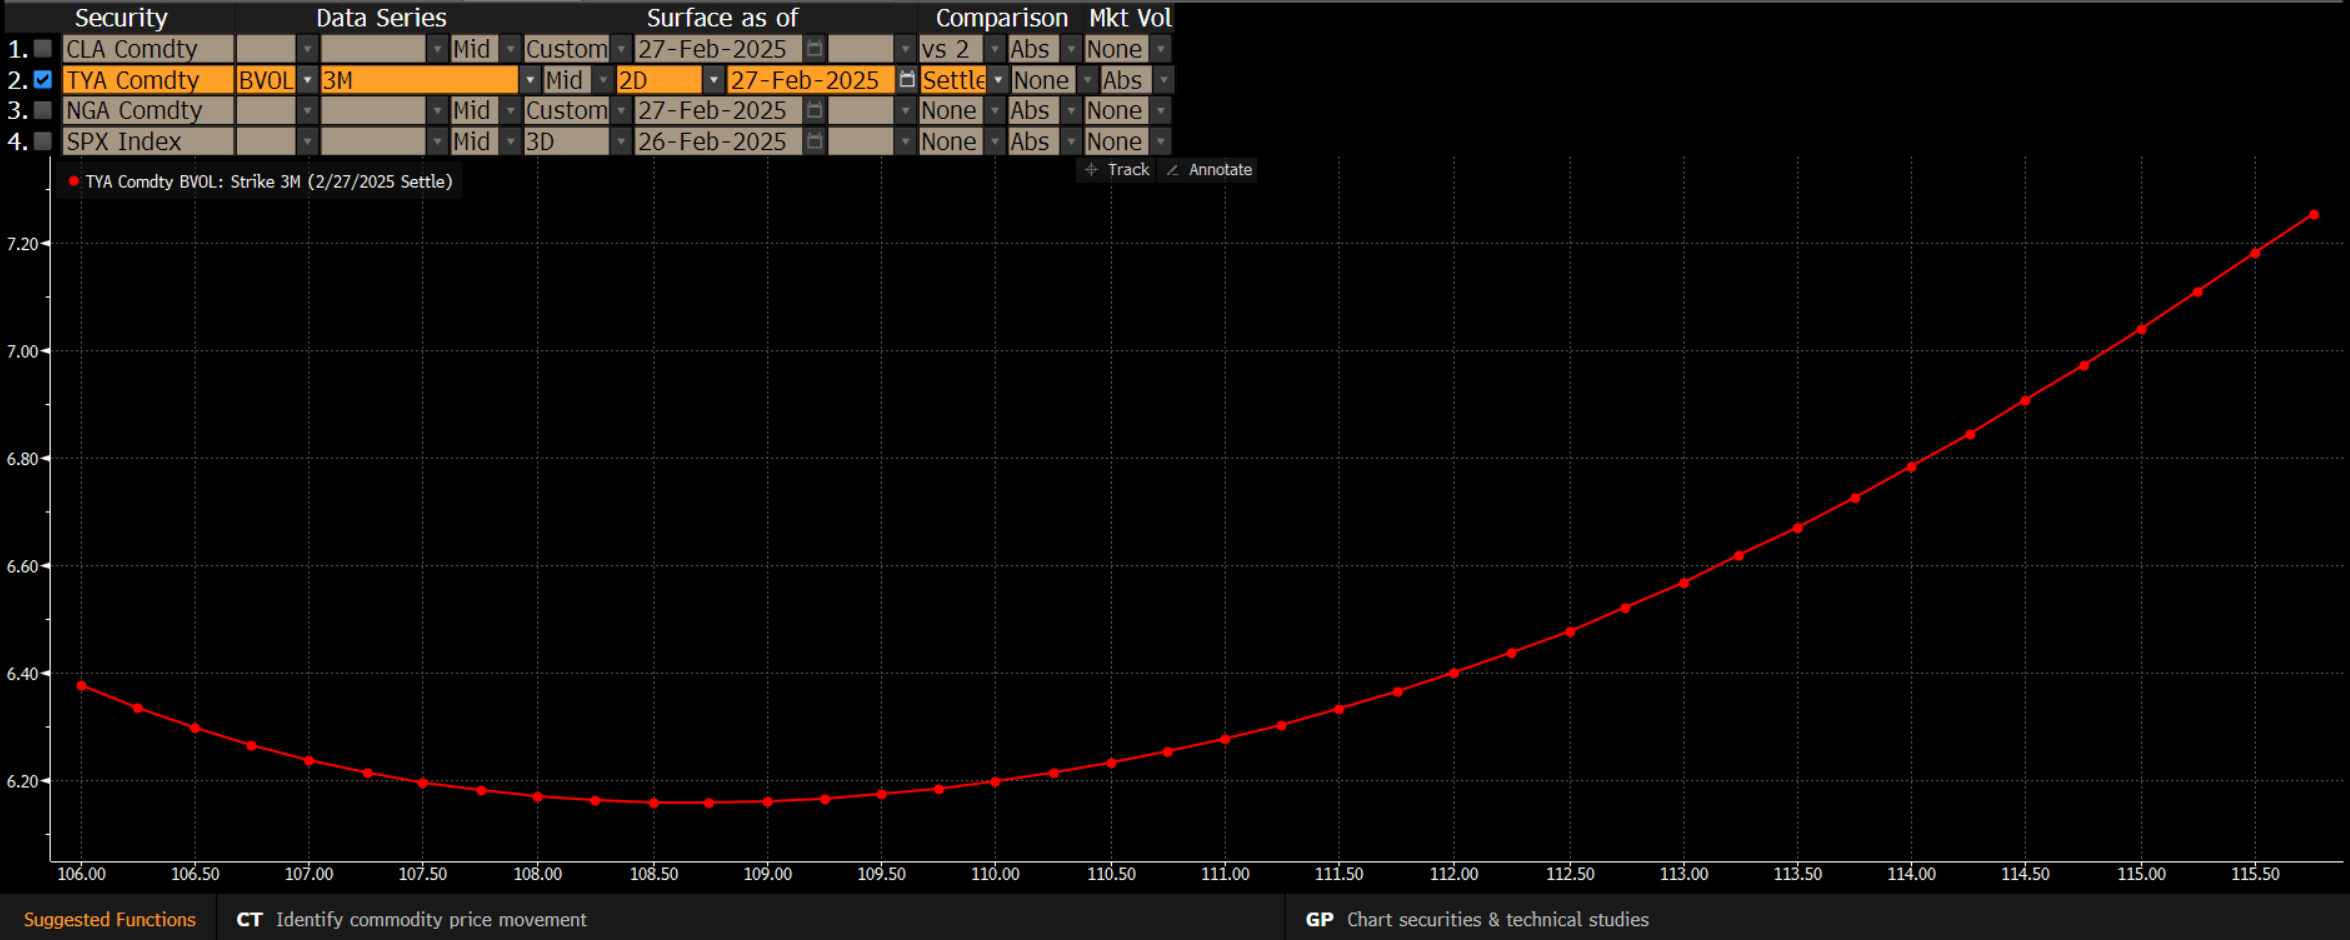
\includegraphics[width=1\textwidth]{Q2_2}
	\end{figure}

\begin{figure}[h]
	\caption{Volatility Surface of \texttt{NGJ5 Comdty}}
	\centering
	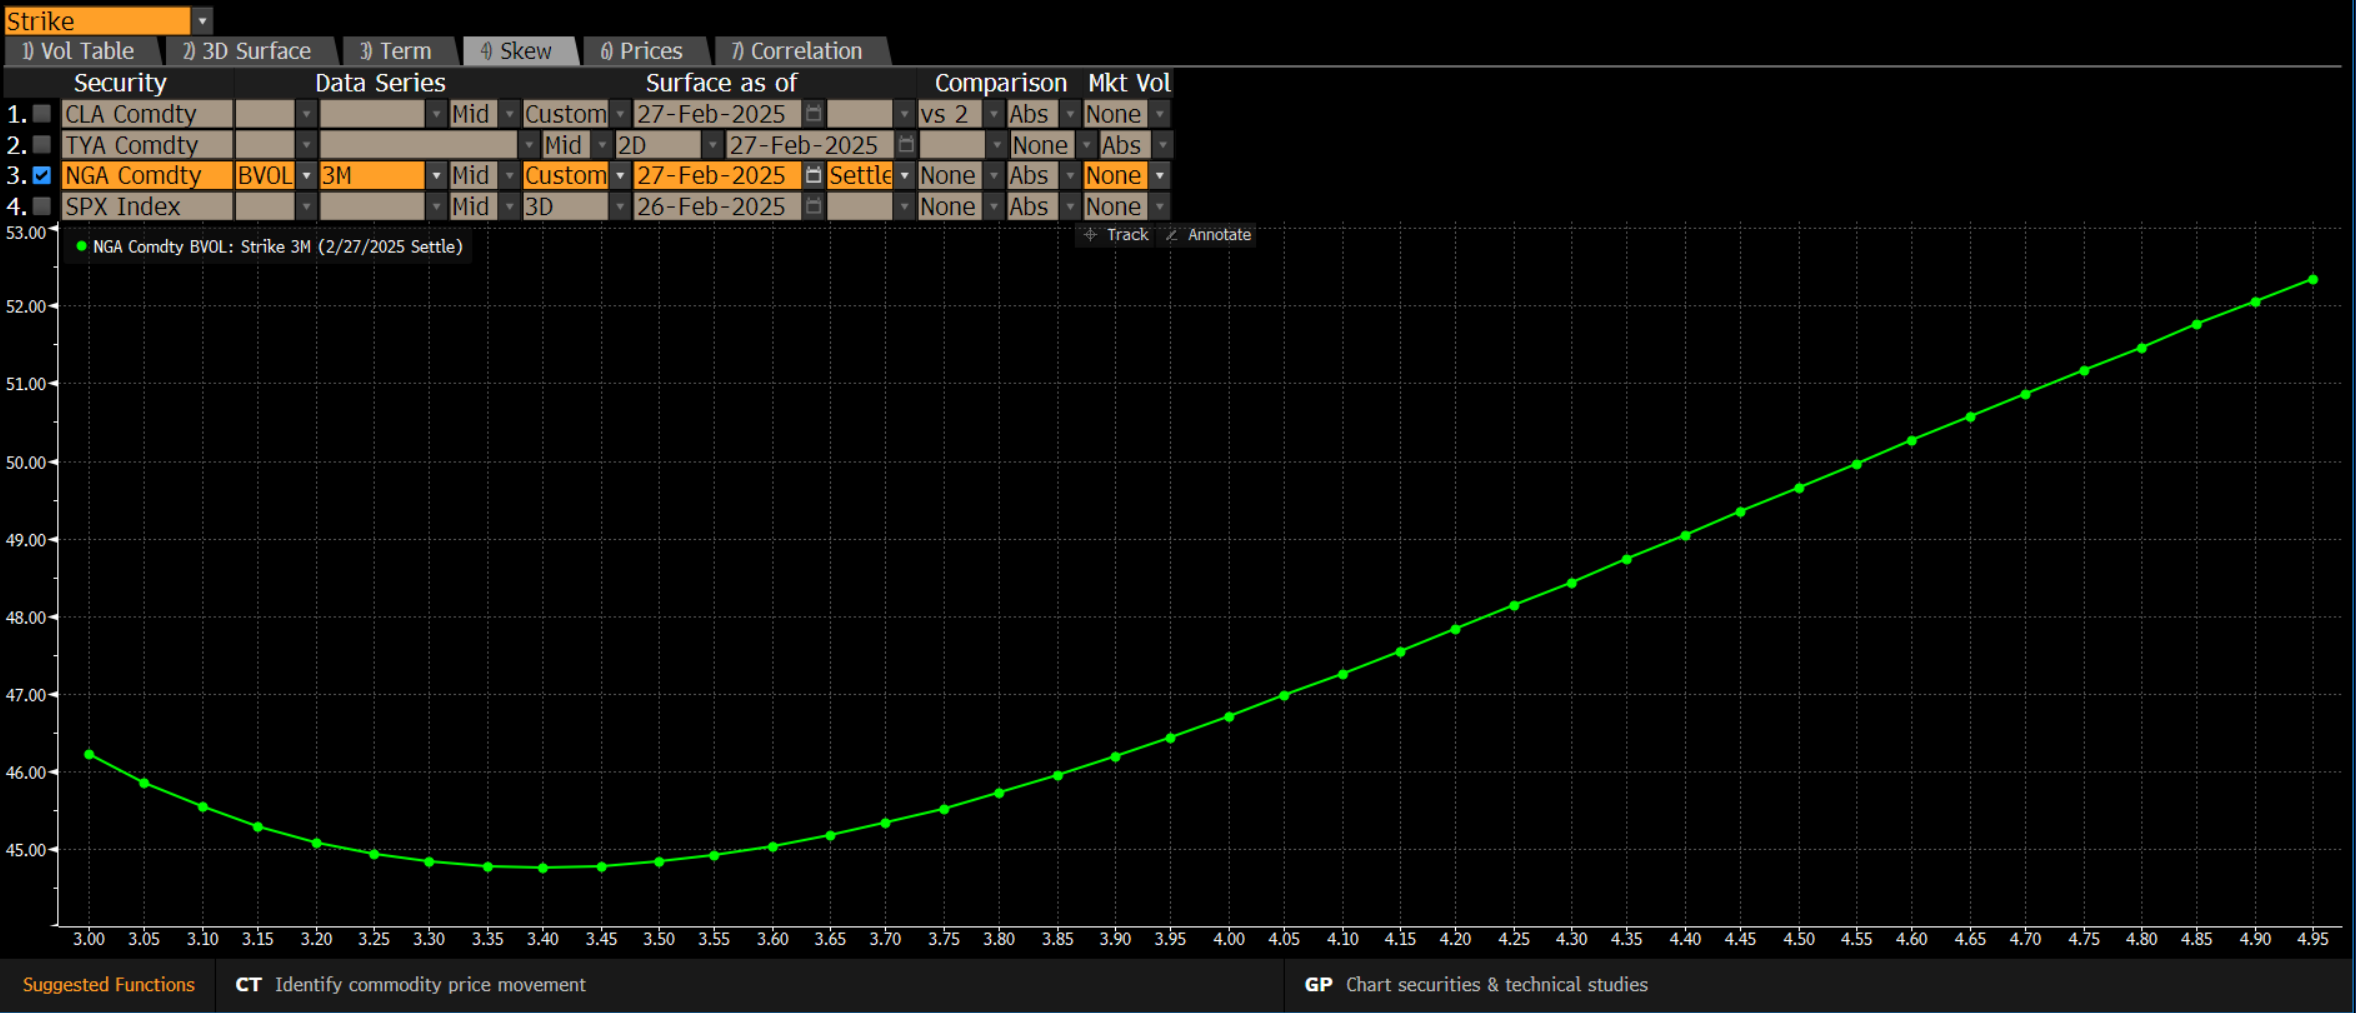
\includegraphics[width=1\textwidth]{Q2_3}
\end{figure}

\clearpage

Here we get a downward sloping graph of \texttt{SPY Equity} and \texttt{ESH5 Index}; typically a  downward-sloping volatility surface in the 3-month range indicates that implied volatility decreases as strike prices increase, reflecting a negative volatility skew. This pattern often signals bearish market sentiment, with investors more concerned about downside risks (e.g., potential price drops) than upside potential. Higher implied volatilities for lower strike prices (out-of-the-money puts) suggest increased demand for downside protection, possibly due to market stress, upcoming events like earnings announcements, or historical patterns of sharp declines. For traders, this skew implies that put options are more expensive, while call options are cheaper, influencing strategies such as put spreads or risk reversals. 

\begin{figure}[h]
	\caption{Volatility Surface of \texttt{SPY Equity}}
	\centering
	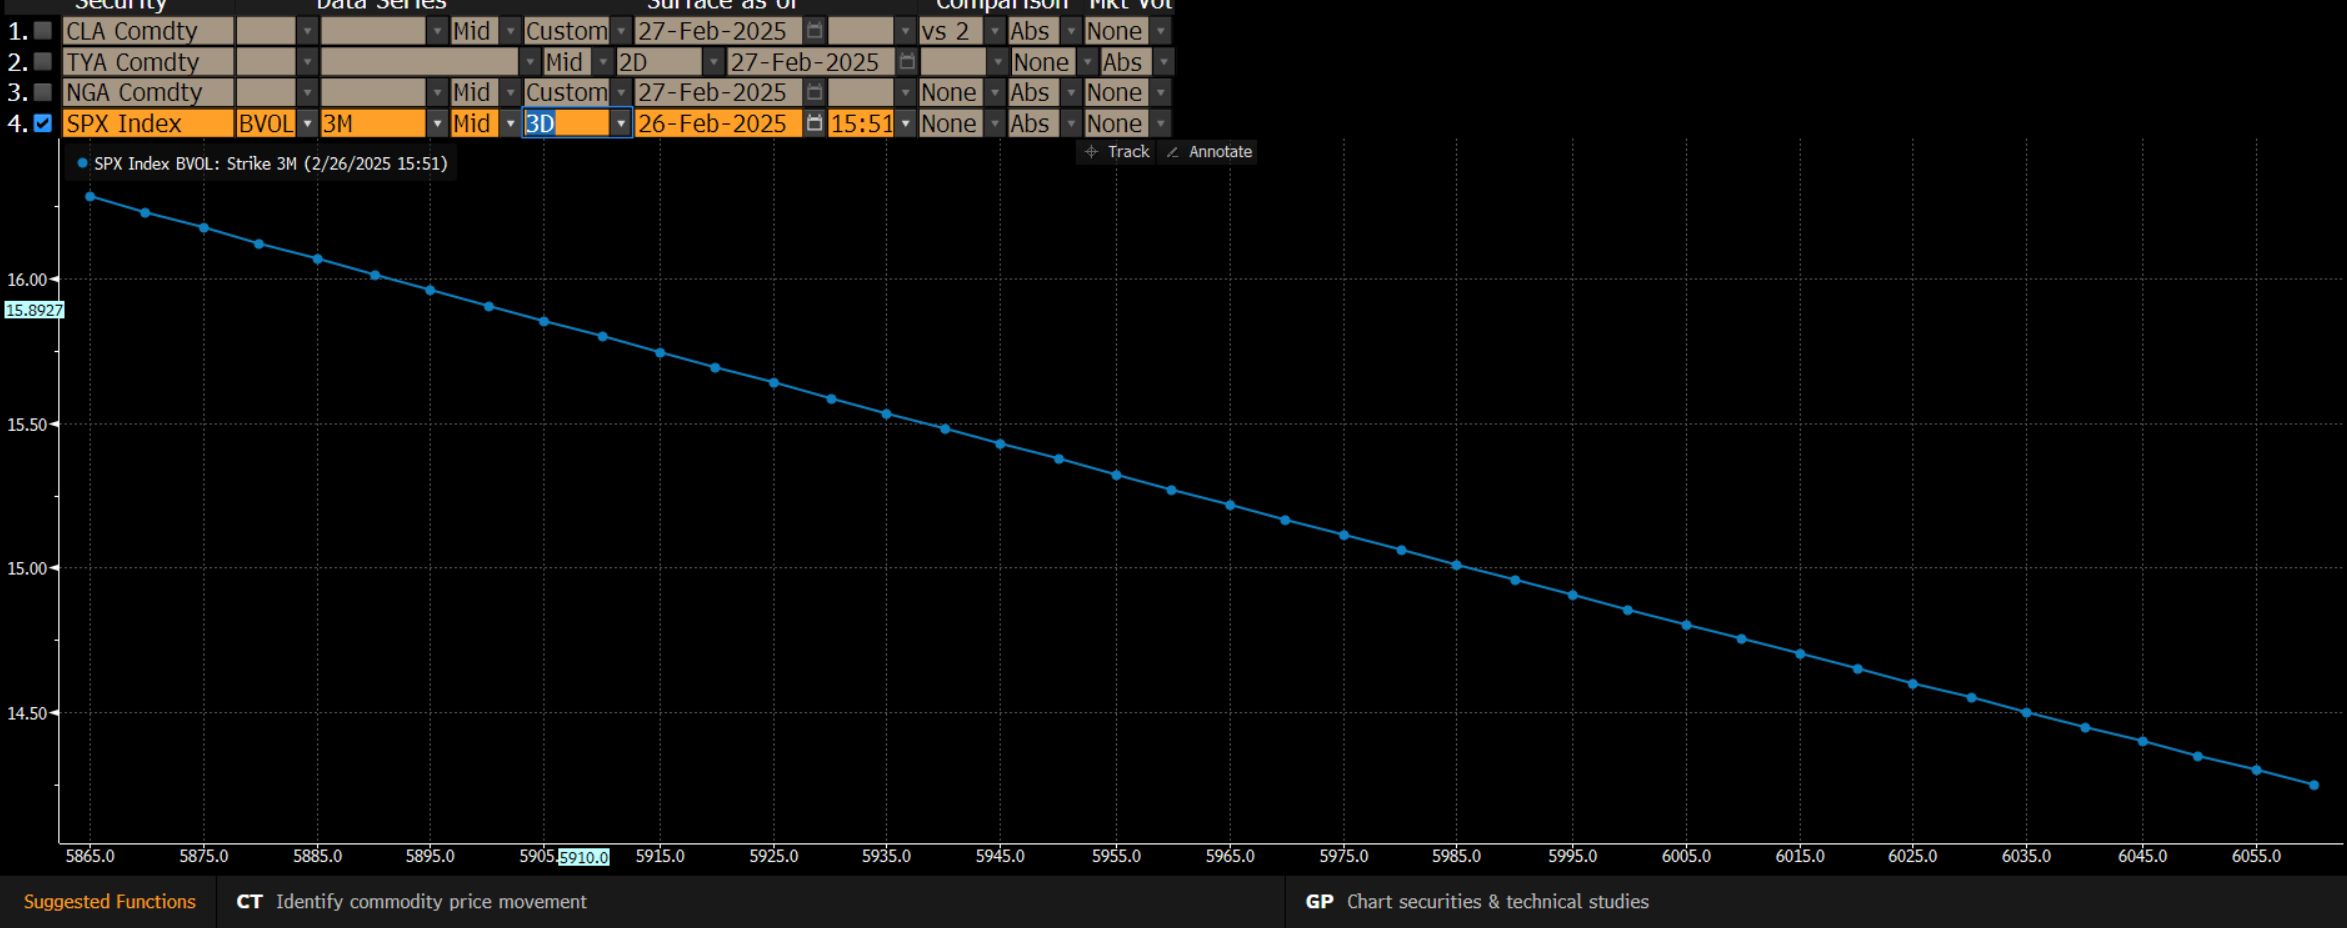
\includegraphics[width=1\textwidth]{Q2_4}
\end{figure}
\begin{figure}[h]
	\caption{Volatility Surface of \texttt{ESH5 Index}}
	\centering
	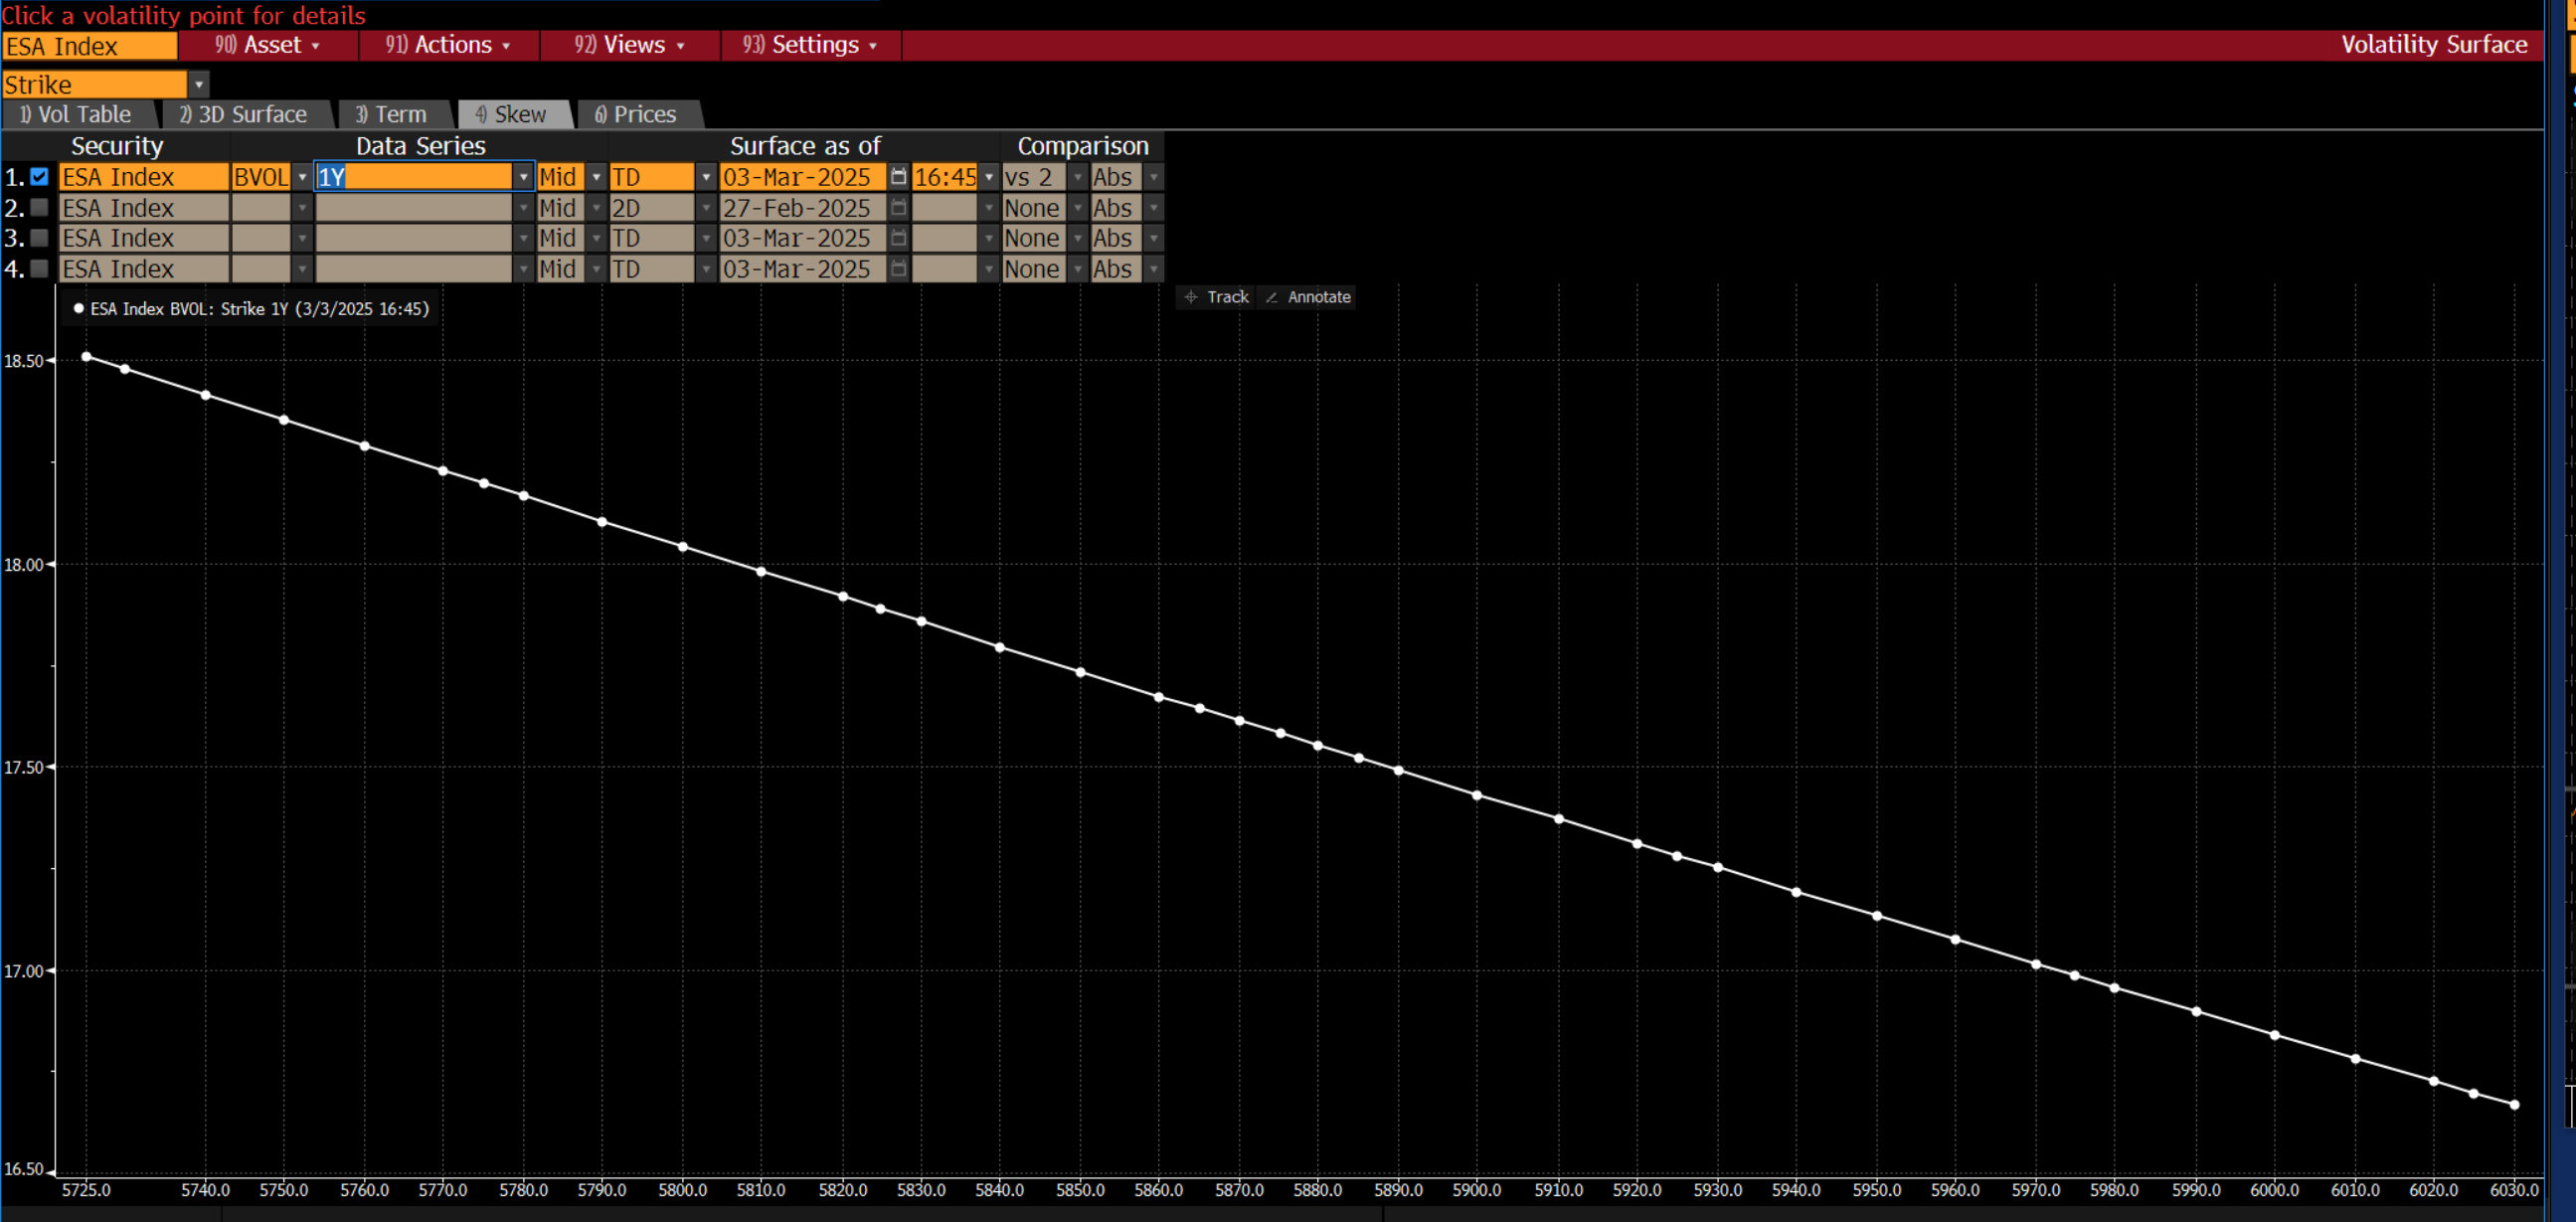
\includegraphics[width=1\textwidth]{Q2_5}
\end{figure}

	\clearpage
	
	\subsection*{Question 3}
	 Suppose the stock price is 70, the risk-free rate is 5\% continuously compounded. What is the price of a 1 year call struck at 70 if the volatility is 0. How would you hedge the call. Check your answer with the option calculator making volatility smaller and smaller.
	 
	 \textbf{Answer}
	 
	 Here I used the integration of Fast Fourier Transformation (FFT) and Fractional Fast Fourier Transformation (FrFFT) for this problem; there are 4 methods to be chosen, GBM, Heston, Variance Gamma, and Black-Scholes. Here I used Black-Scholes.
	 
	 If $\sigma=0$ and there is no dividend in this scenario, the stock price is deterministic and grows at rate $r$. In one year, it is thus worth $70 \cdot e^{0.05} \approx 73.5889$. The strike is $K=70$. Our payoff is thus 3.588. Discounting at rate $r$, we get as today's fair option price $3.588 \cdot e^{-0.05} \approx 3.4139$. When I set \texttt{r = 0.05, q = 0, sigma = 0}, the printout is:
	 
	 \begin{minipage}{\linewidth}
	 	\begin{Verbatim}
     ===================
     Model is BlackScholes
     -------------------
     
     
     Option via Integration: for strike 70.0000 the option premium is 3.4155
     FrFFT execution time was 0.0215478
	 	\end{Verbatim}
	 \end{minipage}
 
    The choice of damping factors, grid truncation error, and numerical integration error may all cause small differences when using Fast Fourier Transformation, but overall the result corresponds with the result we calculated from the Option Pricing Calculator.
 
	 My python codes are as follows:
	 
	 \begin{lstlisting}
     
     import warnings
     warnings.filterwarnings("ignore")
     
     import numpy as np
     import cmath
     import math
     import time
     
     # Fixed Parameters
     S0 = 70
     K = 70
     k = math.log(K)
     r = 0.05
     q = 0
     
     # Parameters for FFT and FrFFT 
     
     n_FFT = 9
     N_FFT = 2**n_FFT
     
     n_FrFFT = 9
     N_FrFFT = 2**n_FrFFT
     
     N = 1000 # it doesn' impact the numerical results if the code is correct 
     
     #step-size
     eta = 0.25
     # damping factor
     alpha = 0.4
     
     # step-size in log strike space
     lda_FFT = (2*math.pi/N_FFT)/eta # lda is fixed under FFT
     lda_FrFFT = 0.001 # lda is an adjustable parameter under FrFFT, 
     
     
     #Choice of beta
     beta = np.log(S0)-N*lda_FFT/2
     #beta = np.log(S0)-N*lda_FrFFT/2
     #beta = np.log(K)
     
     #model-specific Parameters
     model = 'BlackScholes'
     
     params = []     
     if (model == 'GBM'):
     
     sig = 0.3
     params.append(sig);
     
     elif model == 'BlackScholes':  
     sigma = 0  # Volatility  
     params.append(sigma)  
     
     elif (model == 'VG'):
     
     sig = 0.3
     nu = 0.5
     theta = -0.4
     #
     params.append(sig);
     params.append(nu);
     params.append(theta);
     
     
     
     elif (model == 'Heston'):
     
     kappa = 2.0
     theta = 0.05
     sig = 0.30
     rho = -0.70
     v0 = 0.04
     #
     params.append(kappa)
     params.append(theta)
     params.append(sig)
     params.append(rho)
     params.append(v0)
     
     def generic_CF(u, params, S0, r, q, T, model):
     
     if (model == 'GBM'):
     
     sig = params[0]
     mu = np.log(S0) + (r-q-sig**2/2)*T
     a = sig*np.sqrt(T)
     phi = np.exp(1j*mu*u-(a*u)**2/2)
     
     elif (model == 'BlackScholes'):
     sigma = params[0]  # Volatility
     
     mu = np.log(S0) + (r - q - 0.5 * sigma**2) * T  # Drift
     a = sigma * np.sqrt(T)  # Standard deviation over the maturity period
     phi = np.exp(1j * mu * u - 0.5 * a**2 * u**2)  # Characteristic function for Black-Scholes
     
     
     elif(model == 'Heston'):
     
     kappa  = params[0]
     theta  = params[1]
     sigma  = params[2]
     rho    = params[3]
     v0     = params[4]
     
     tmp = (kappa-1j*rho*sigma*u)
     g = np.sqrt((sigma**2)*(u**2+1j*u)+tmp**2)
     
     pow1 = 2*kappa*theta/(sigma**2)
     
     numer1 = (kappa*theta*T*tmp)/(sigma**2) + 1j*u*T*r + 1j*u*math.log(S0)
     log_denum1 = pow1 * np.log(np.cosh(g*T/2)+(tmp/g)*np.sinh(g*T/2))
     tmp2 = ((u*u+1j*u)*v0)/(g/np.tanh(g*T/2)+tmp)
     log_phi = numer1 - log_denum1 - tmp2
     phi = np.exp(log_phi)
     
     #g = np.sqrt((kappa-1j*rho*sigma*u)**2+(u*u+1j*u)*sigma*sigma)
     #beta = kappa-rho*sigma*1j*u
     #tmp = g*T/2
     
     #temp1 = 1j*(np.log(S0)+(r-q)*T)*u + kappa*theta*T*beta/(sigma*sigma)
     #temp2 = -(u*u+1j*u)*v0/(g/np.tanh(tmp)+beta)
     #temp3 = (2*kappa*theta/(sigma*sigma))*np.log(np.cosh(tmp)+(beta/g)*np.sinh(tmp))
     
     #phi = np.exp(temp1+temp2-temp3);
     
     
     elif (model == 'VG'):
     
     sigma  = params[0];
     nu     = params[1];
     theta  = params[2];
     
     if (nu == 0):
     mu = np.log(S0) + (r-q - theta -0.5*sigma**2)*T
     phi  = np.exp(1j*u*mu) * np.exp((1j*theta*u-0.5*sigma**2*u**2)*T)
     else:
     mu  = np.log(S0) + (r-q + np.log(1-theta*nu-0.5*sigma**2*nu)/nu)*T
     phi = np.exp(1j*u*mu)*((1-1j*nu*theta*u+0.5*nu*sigma**2*u**2)**(-T/nu))
     
     return phi
     def evaluateIntegral(params, S0, K, r, q, T, alpha, eta, N, model):
     
     # Just one strike at a time
     # no need for Fast Fourier Transform
     
     # discount factor
     df = math.exp(-r*T)
     
     sum1 = 0
     for j in range(N):
     nuJ = j*eta
     psi_nuJ = df*generic_CF(nuJ-(alpha+1)*1j, params, S0, r, q, T, model)/((alpha + 1j*nuJ)*(alpha+1+1j*nuJ))
     if j == 0:
     wJ = (eta/2)
     else:
     wJ = eta
     sum1 += np.exp(-1j*nuJ*k)*psi_nuJ*wJ
     
     cT_k = (np.exp(-alpha*k)/math.pi)*sum1
     
     return np.real(cT_k) 
     
     def genericFFT(params, S0, K, r, q, T, alpha, eta, n, model):
     
     N = 2**n
     
     # step-size in log strike space
     lda = (2*np.pi/N)/eta
     
     #Choice of beta
     #beta = np.log(S0)-N*lda/2
     #beta = np.log(K)
     
     # forming vector x and strikes km for m=1,...,N
     km = np.zeros((N))
     xX = np.zeros((N))
     
     # discount factor
     df = math.exp(-r*T)
     
     nuJ = np.arange(N)*eta
     psi_nuJ = generic_CF(nuJ-(alpha+1)*1j, params, S0, r, q, T, model)/((alpha + 1j*nuJ)*(alpha+1+1j*nuJ))
     
     for j in range(N):  
     km[j] = beta+j*lda
     if j == 0:
     wJ = (eta/2)
     else:
     wJ = eta
     
     xX[j] = np.exp(-1j*beta*nuJ[j])*df*psi_nuJ[j]*wJ
     
     yY = np.fft.fft(xX)
     cT_km = np.zeros((N))  
     for i in range(N):
     multiplier = np.exp(-alpha*km[i])/math.pi
     cT_km[i] = multiplier*np.real(yY[i])
     
     return km, cT_km
     
     def genericFrFFT(params, S0, K, r, q, T, alpha, eta, n, lda, model):
     
     N = 2**n
     gamma = eta*lda/(2*math.pi)
     
     #Choice of beta
     #beta = np.log(S0)-N*lda/2
     beta = np.log(K)
     
     # initialize x, y, z, and cT_km
     km = np.zeros((N))
     x = np.zeros((N))
     y = np.zeros((2*N), dtype=np.complex128)
     z = np.zeros((2*N), dtype=np.complex128)
     cT_km = np.zeros((N)) 
     
     # discount factor
     df = math.exp(-r*T)
     
     # compute x
     nuJ = np.arange(N)*eta
     psi_nuJ = generic_CF(nuJ-(alpha+1)*1j, params, S0, r, q, T, model)/((alpha + 1j*nuJ)*(alpha+1+1j*nuJ))
     
     for j in range(N):  
     km[j] = beta+j*lda
     if j == 0:
     wJ = (eta/2)
     else:
     wJ = eta
     x[j] = np.exp(-1j*beta*nuJ[j])*df*psi_nuJ[j]*wJ
     
     # set up y
     for i in range(N):
     y[i] = np.exp(-1j*math.pi*gamma*i**2)*x[i]
     y[N:] = 0
     
     # set up z
     for i in range(N):
     z[i] = np.exp(1j*math.pi*gamma*i**2)
     z[N:] = z[:N][::-1]
     
     # compute xi_hat
     xi_hat = np.fft.ifft(np.fft.fft(y) * np.fft.fft(z))
     
     # compute call prices
     for i in range(N):
     cT_km[i] = np.exp(-alpha*(beta + i*lda))/math.pi * (np.exp(-1j*math.pi*gamma*i**2)*xi_hat[i]).real
     
     return km, cT_km
     
     print(' ')
     print('===================')
     print('Model is %s' % model)
     print('-------------------')
     
     T = 1
     
     # FFT
     print(' ')
     start_time = time.time()
     km, cT_km = genericFFT(params, S0, K, r, q, T, alpha, eta, n_FFT, model)
     #cT_k = cT_km[0]
     cT_k = np.interp(k, km, cT_km)
     
     elapsed_time = time.time() - start_time
     
     #cT_k = np.interp(np.log(k), km, cT_km)
     print("Option via FFT: for strike %s the option premium is %6.4f" % (np.exp(k), cT_k))
     #print("Option via FFT: for strike %s the option premium is %6.4f" % (np.exp(k), cT_km[0]))
     print('FFT execution time was %0.7f' % elapsed_time)
     
     # FrFFT
     print(' ')
     start_time = time.time()
     km, cT_km = genericFrFFT(params, S0, K, r, q, T, alpha, eta, n_FrFFT, lda_FrFFT, model)
     #cT_k = cT_km[0]
     cT_k = np.interp(k, km, cT_km)
     
     elapsed_time = time.time() - start_time
     
     #cT_k = np.interp(np.log(), km, cT_km)
     print("Option via FrFFT: for strike %s the option premium is %6.4f" % (np.exp(k), cT_k))
     #print("Option via FFT: for strike %s the option premium is %6.4f" % (np.exp(k), cT_km[0]))
     print('FrFFT execution time was %0.7f' % elapsed_time)
     
     
     # Integral
     print(' ')
     start_time = time.time()
     cT_k = evaluateIntegral(params, S0, K, r, q, T, alpha, eta, N, model)
     elapsed_time = time.time() - start_time
     print("Option via Integration: for strike %s the option premium is %6.4f" % (np.exp(k), cT_k))
     print('Evaluation of integral time was %0.7f' % elapsed_time)
	 	
	 \end{lstlisting}
 
 Then I double checked it from the option price calculator:
 
     \begin{figure}[h]
    	\caption{Results from Option Calculator}
    	\centering
    	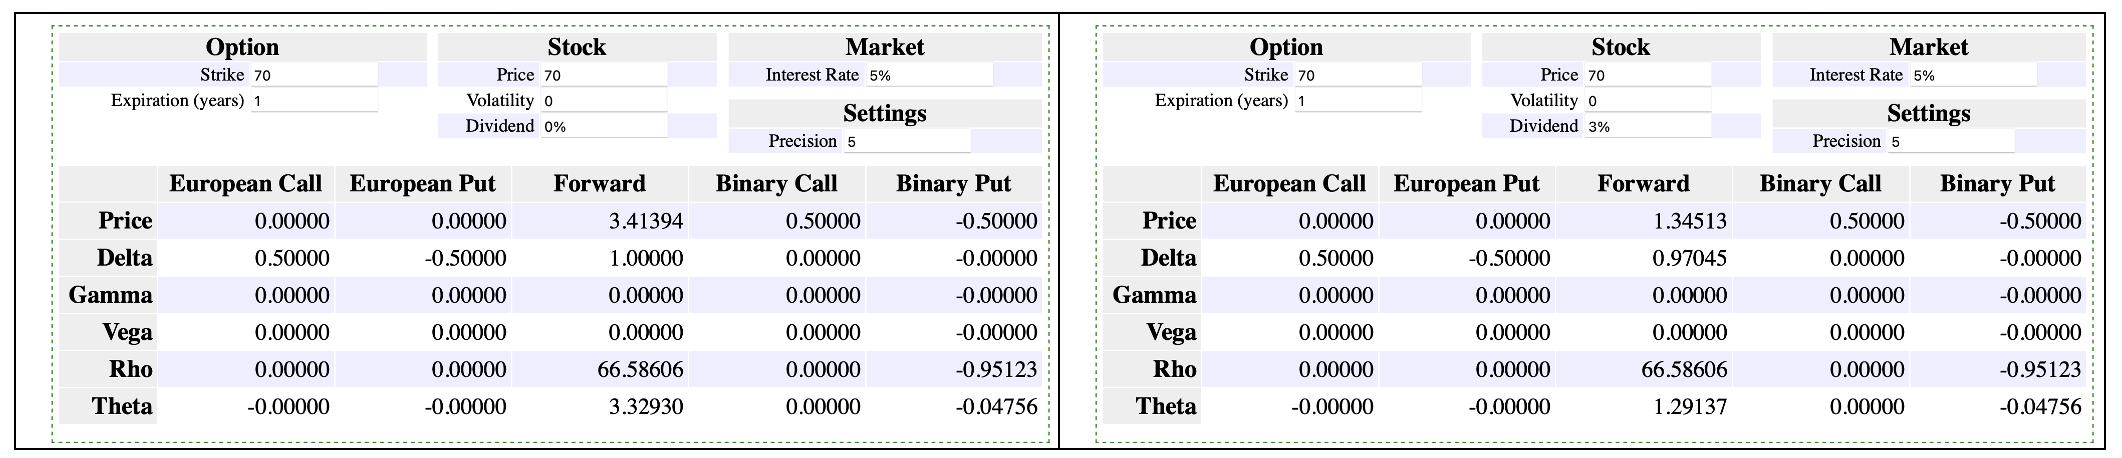
\includegraphics[width=1\textwidth]{Q3}
    \end{figure}
  
  
  \clearpage
	 
	 \subsection*{Question 4}
	 Explain why an American option on a stock paying continuous dividend yield is always worth as much as its intrinsic value. Give a numerical example of a situation when European option is worth less than intrinsic value. (Give the numerical value of stock price, strike price, time to expiration, etc.)
	 
	 \textbf{Answer}
	 
	 \textbf{Concept}
	 
	 Intrinsic value of a call option is the difference between the current price of the underlying asset and the strike price of the option, if the underlying asset's price is above the strike price. If the underlying asset's price is below the strike price, the call option has no intrinsic value. Thus it can be expressed as:
	 
	  \[
	 \max(S - K, 0)
	 \]
	 
	 Here we have \( S \) to be the current stock price, and \( K \) to be the strike price
	 
	If the stock pays a continuous dividend yield, the stock price is expected to decrease as dividends are paid. This increases the incentive to exercise the call option early to avoid losing value from future dividends. Since the American option can be exercised early, the holder will exercise it if the intrinsic value exceeds the option’s continuation value (the value of holding the option). Therefore, the American option is always worth at least its intrinsic value.
	 
	 \textbf{Numerical Example}
	 
	  For a the numerical example, we can set:
	 \begin{itemize}
	 	\item Stock price: \( S = 100 \)
	 	\item Strike price: \( K = 90 \)
	 	\item Time to expiration: 1 year
	 	\item Risk-free interest rate: 5\%
	 	\item Continuous dividend yield: 3\%
	 	\item Volatility: 20\%
	 \end{itemize}
	 
	 Using the Black-Scholes formula, the European call option price is approximately:
	 
	 \[
	 C_{\text{European}} = 12.03
	 \]
	 
	 \begin{tcolorbox}[width=\linewidth, colframe=MidnightBlue, title=Calculation of $C_{\text{European}}$]
	 	
	 	We have the Black-Scholes Formula:
	 	\[
	 	C = S e^{-qt} N(d_1) - K e^{-rt} N(d_2)
	 	\]
	 	
	 	Where \( d_1 \) and \( d_2 \) can be calculated as:
	 	
	 	\[
	 	d_1 = \frac{\ln\left(\frac{S}{K}\right) + (r - q + \frac{\sigma^2}{2})t}{\sigma\sqrt{t}}
	 	\]
	 	
	 	\[
	 	d_2 = d_1 - \sigma\sqrt{t}
	 	\]
	 	
	 	Given what we previously set: \( S = 100 \), \( K = 90 \), \( r = 0.05 \), \( q = 0.03 \), \( \sigma = 0.20 \), \( t = 1 \):
	 	
	 	\[
	 	d_1 = \frac{\ln(100/90) + (0.05 - 0.03 + 0.5(0.2^2))(1)}{0.2\sqrt{1}} = \frac{\ln(1.1111) + (0.02 + 0.02)}{0.2}= \frac{0.1054 + 0.04}{0.2} = \frac{0.1454}{0.2} = 0.727
	 	\]
	 	
	 	\[
	 	d_2 = 0.727 - 0.2 = 0.527
	 	\]
	 	
	 	Then we can find \( N(d_1) \) and \( N(d_2) \) using standard normal distribution tables:
	 	
	 	\[
	 	N(0.727) \approx 0.7673
	 	\]
	 	
	 	\[
	 	N(0.527) \approx 0.7014
	 	\]
	 	
	 Finally we plug them back into the Black-Scholes Formula
	 	
	 	\[
	 	C = 100 e^{-0.03(1)}(0.7673) - 90 e^{-0.05(1)}(0.7014) = 100(0.9704)(0.7673) - 90(0.9512)(0.7014)
	 	\]
	 	
	 	\[
	 	C = 74.43 - 60.91  \approx 12.03
	 	\]
	 	
	 \end{tcolorbox}
 
	 The intrinsic value is:
	 
	 \[
	 S - K = 100 - 90 = 10
	 \]
	 
	 Here, the European option is worth 12.03, which is greater than the intrinsic value because there is still time value.

	 
	 Then we modify the example:
	 
	 \begin{itemize}
	 \item Stock price: \( S = 100 \)
	 \item Strike price: \( K = 110 \) (out of the money)
	 \item Time to expiration: 1 month
	 \item Dividend yield: 3\%
	 \item Volatility: 10\%
	\end{itemize}
	 
	 Using Black-Scholes and similar calculation as previous step:
	 
	 \[
	 C_{\text{European}} \approx 0.25
	 \]
	 
	 But the intrinsic value is:
	 
	 \[
	 \max(100 - 110, 0) = 0
	 \]
	 
	 In this case, the European option is worth less than its intrinsic value, because there is no early exercise opportunity, and the option is out of the money.
	 
	 \clearpage
	 
	 \subsection*{Question 5}
	 Explain the European call-put parity argument. Why it can not be used for American options
	 
	 \textbf{Answer}
	 
	 The Put-Call Parity is a fundamental relationship between the prices of European call and put options on the same underlying asset, with the same strike price and expiration date. It defines a relationship between the price of a European call option and European put option, both with the identical strike price and expiry, namely that a portfolio of a long call option and a short put option is equivalent to (and hence has the same value as) a single forward contract at this strike price and expiry
	 
	 The formula is:
	 
	 \[
	 C - P = S e^{-qt} - K e^{-rt}
	 \]
	 
	 \begin{itemize}
	 	\item \( C \): Price of the European call option
	 	\item \( P \): Price of the European put option
	 	\item \( S \): Current stock price
	 	\item \( K \): Strike price
	 	\item \( r \): Risk-free interest rate
	 	\item \( q \): Continuous dividend yield
	 	\item \( t \): Time to expiration
	 	\item \( e^{-qt} \): Discounted stock price due to dividend payments
	 	\item \( e^{-rt} \): Discounted strike price due to risk-free rate
	 \end{itemize}

	 The parity works well for European options because they can only be exercised at expiration. The key idea behind this formula is that a portfolio consisting of a long European call option and a short European put option is equivalent to holding the underlying stock while borrowing the present value of the strike price.
	 
	 Both portfolios will yield the same payoff at expiration, which is why they must have the same value before expiration (by the no-arbitrage principle).
	 

	 However, the Put-Call Parity does not directly apply to American options because:
	 
	 \begin{itemize}
	 \item American options can be exercised at any time before expiration, which adds an additional layer of complexity. This early exercise possibility makes the payoff structure of American options different from European options.

	 \item For American call options on dividend-paying stocks, early exercise is often optimal just before the ex-dividend date (to avoid losing dividends). This means the American call option might be more valuable than the European call option.
	 
	 \item Unlike European options, American calls and puts do not have a fixed parity relationship because the option holder’s decision to exercise early can affect the option's price.
	 
	 \item The strict no-arbitrage condition that holds for European options does not necessarily apply to American options due to the early exercise feature. This creates pricing discrepancies that do not align with put-call parity.
	 
	\end{itemize}
	 
	  \begin{tcolorbox}[width=\linewidth, colframe=MidnightBlue, title=A Numerical Example]
	 Suppose we take stock price \( S = 100 \), strike price \( K = 95 \), time to expiration as 6 months, risk-free rate as 5\%, dividend yield as 2\%, European call price 8 and European put price to be 3.
	 
	 \[
	 8 - 3 = 100 e^{-0.02(0.5)} - 95 e^{-0.05(0.5)}
	 \]
	 
	 \[
	 5 = 100(0.9900) - 95(0.9753)
	 \]
	 
	 \[
	 5 = 99 - 92.65
	 \]
	 
	 \[
	 5 = 6.35
	 \]
	 
	 There is a small difference due to rounding, but the parity approximately holds.
	 \end{tcolorbox}
	 
	 \subsection*{Question 6}
	 Calculate the implied volatility of Microsoft stock using March 2025 calls expiring March 21, 2025 with strike 410 and with strike 420. Get the quotes from any data provider, for example, finance.yahoo.com and use all other necessary data. On Bloomberg type \texttt{MSFT Equity CALL} (page down as needed).
	 
	 \textbf{Answer}
	 
	 I used python to calculate the implied volatility. Currently the risk-free rate is 4.24\% as I got from the  \href{https://ycharts.com/indicators/10_year_treasury_rate}{source}. And the current market price for strike 410 is \$3.04 and 420 \$1.21 separately. Then use the Black-Scholes model to recalculate the implied volatility:
	 
	 \begin{lstlisting}
     import numpy as np
     from scipy.stats import norm
     
     # Black-Scholes call option pricing formula
     def black_scholes_call(S, K, T, r, sigma, q=0):
     d1 = (np.log(S / K) + (r - q + 0.5 * sigma ** 2) * T) / (sigma * np.sqrt(T))
     d2 = d1 - sigma * np.sqrt(T)
     return np.exp(-q * T) * S * norm.cdf(d1) - K * np.exp(-r * T) * norm.cdf(d2)
     
     # Implied Volatility Function using Newton-Raphson Method
     def implied_volatility(S, K, T, r, market_price, q=0, tol=1e-6, max_iter=100):
     sigma = 0.2  # Initial Guess
     for i in range(max_iter):
     price = black_scholes_call(S, K, T, r, sigma, q)
     vega = S * np.exp(-q * T) * norm.pdf((np.log(S / K) + (r - q + 0.5 * sigma ** 2) * T) / (sigma * np.sqrt(T))) * np.sqrt(T)
     price_diff = price - market_price
     if abs(price_diff) < tol:
     return sigma
     sigma -= price_diff / vega
     raise ValueError("Implied volatility did not converge")
     
     # Example Inputs
     S = 394.9       # Current stock price (MSFT)
     K = 420           # Strike price, 410 and 420
     T = 18 / 365      # Time to expiration in years, March 21-3
     r = 0.0424        # Risk-free interest rate, get from website
     q = 0.0085         # Continuous dividend yield
     market_price = 1.21 # Call option market price
     
     try:
     iv = implied_volatility(S, K, T, r, market_price, q)
     print(f"Implied Volatility: {iv:.4f}")
     except ValueError as e:
     print(e)
     
	 \end{lstlisting}
 
 And the printout for strike price 410 is
 
 \begin{minipage}{\linewidth}
 	\begin{Verbatim}
     Implied Volatility: 0.2335
 	\end{Verbatim}
 \end{minipage}
	 
 And the printout for strike price 420 is
 
	 \begin{minipage}{\linewidth}
	 	\begin{Verbatim}
     Implied Volatility: 0.2289
	 	\end{Verbatim}
	 \end{minipage}
 
 
	 And I also tested it from the calculator
	 
	 \begin{figure}[h]
	 	\caption{Results using Calculator}
	 	\centering
	 	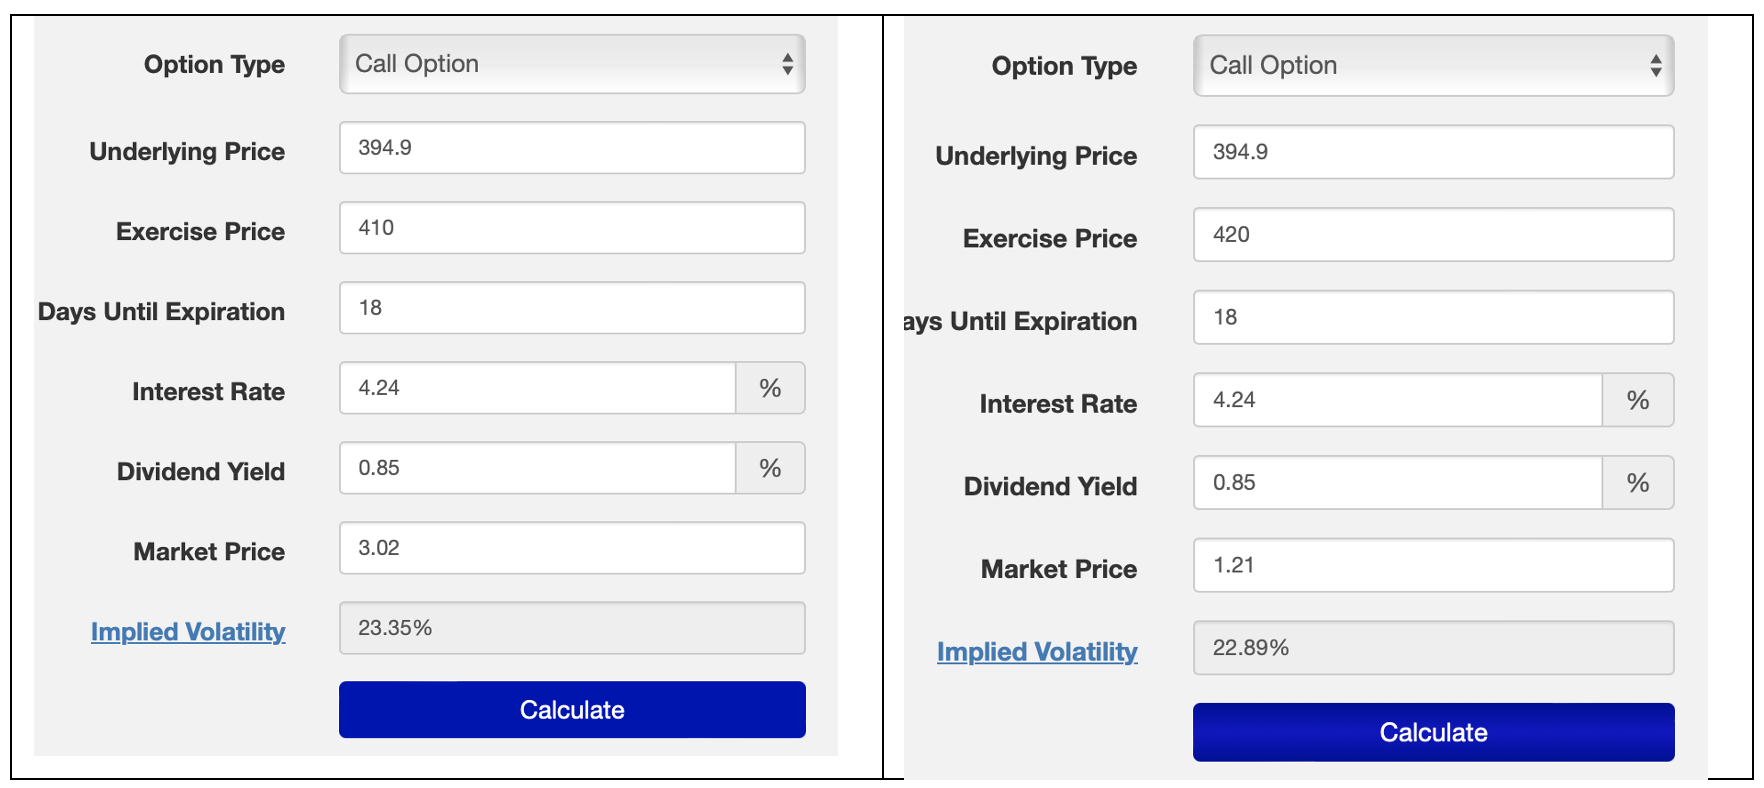
\includegraphics[width=0.8\textwidth]{Q6_3}
	 \end{figure}
 
	 This can be reconfirmed with the data from Yahoo Finance: 
	 
	 \begin{figure}[h]
	 	\caption{Strike Price 410, Expire Date 2025-03-21}
	 	\centering
	 	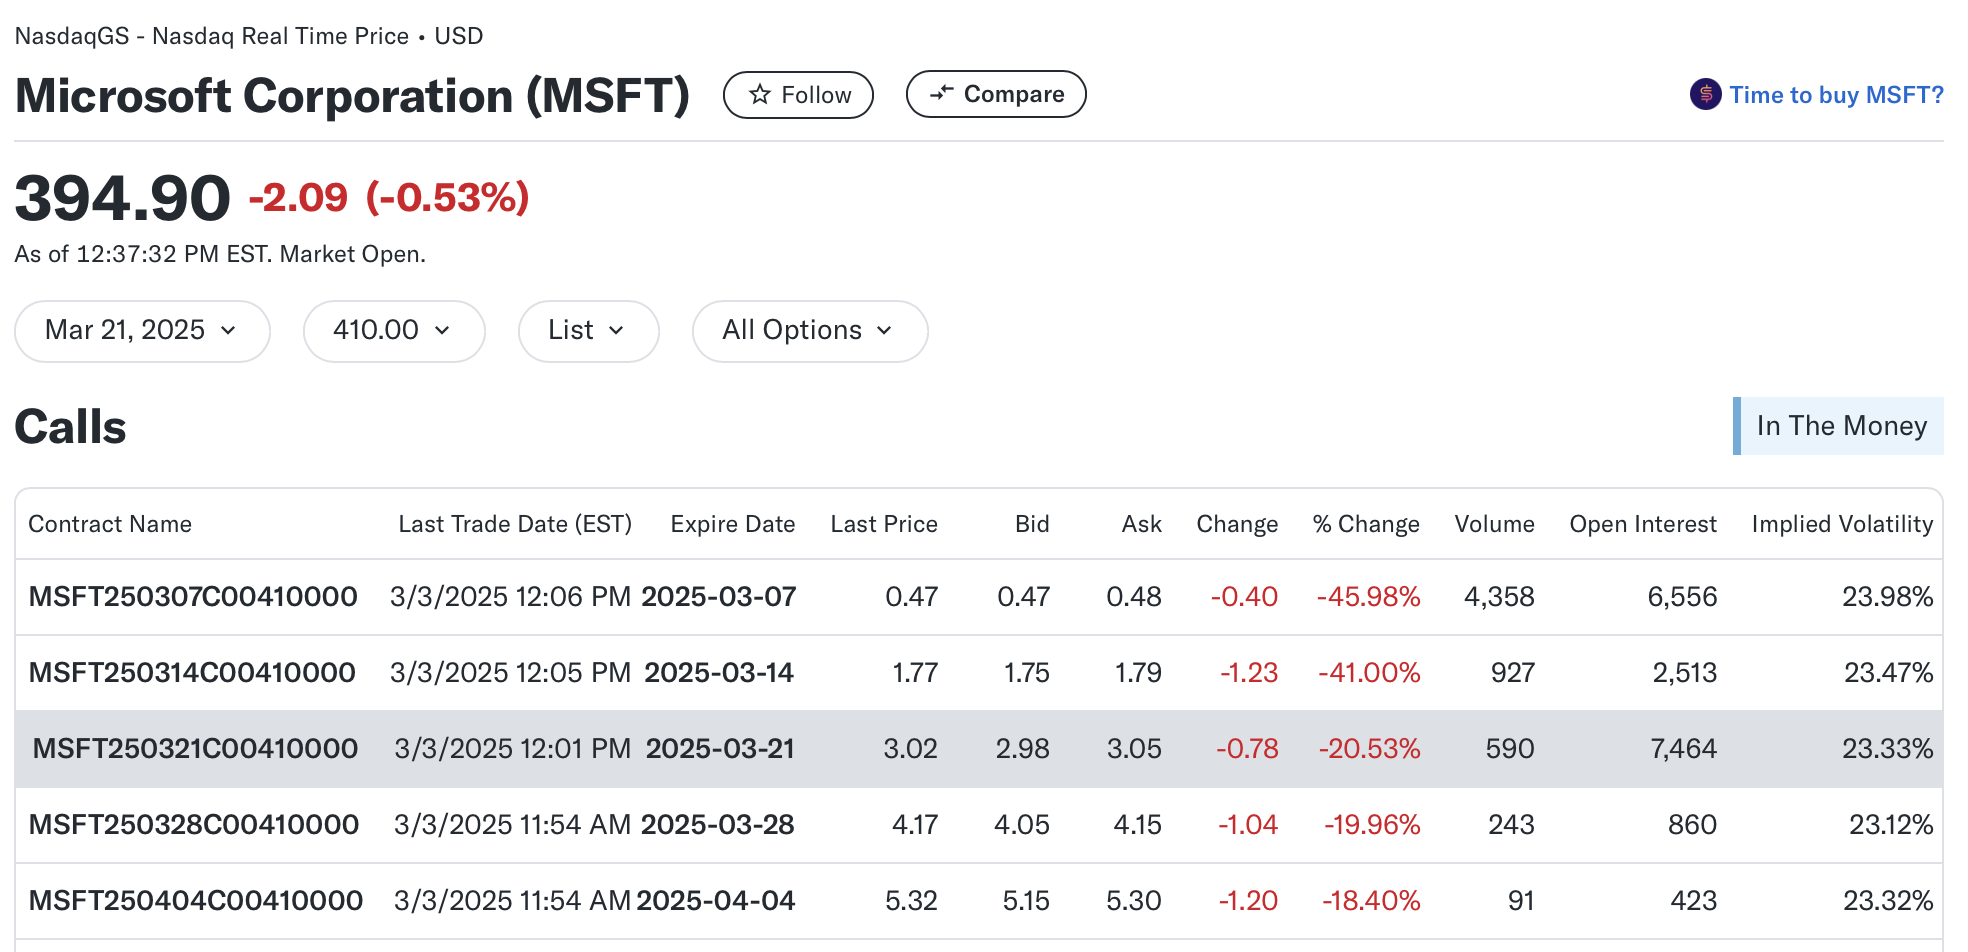
\includegraphics[width=0.9\textwidth]{Q6_1}
	 \end{figure}
	 
	 \begin{figure}[h]
	 	\caption{Strike Price 420, Expire Date 2025-03-21}
	 	\centering
	 	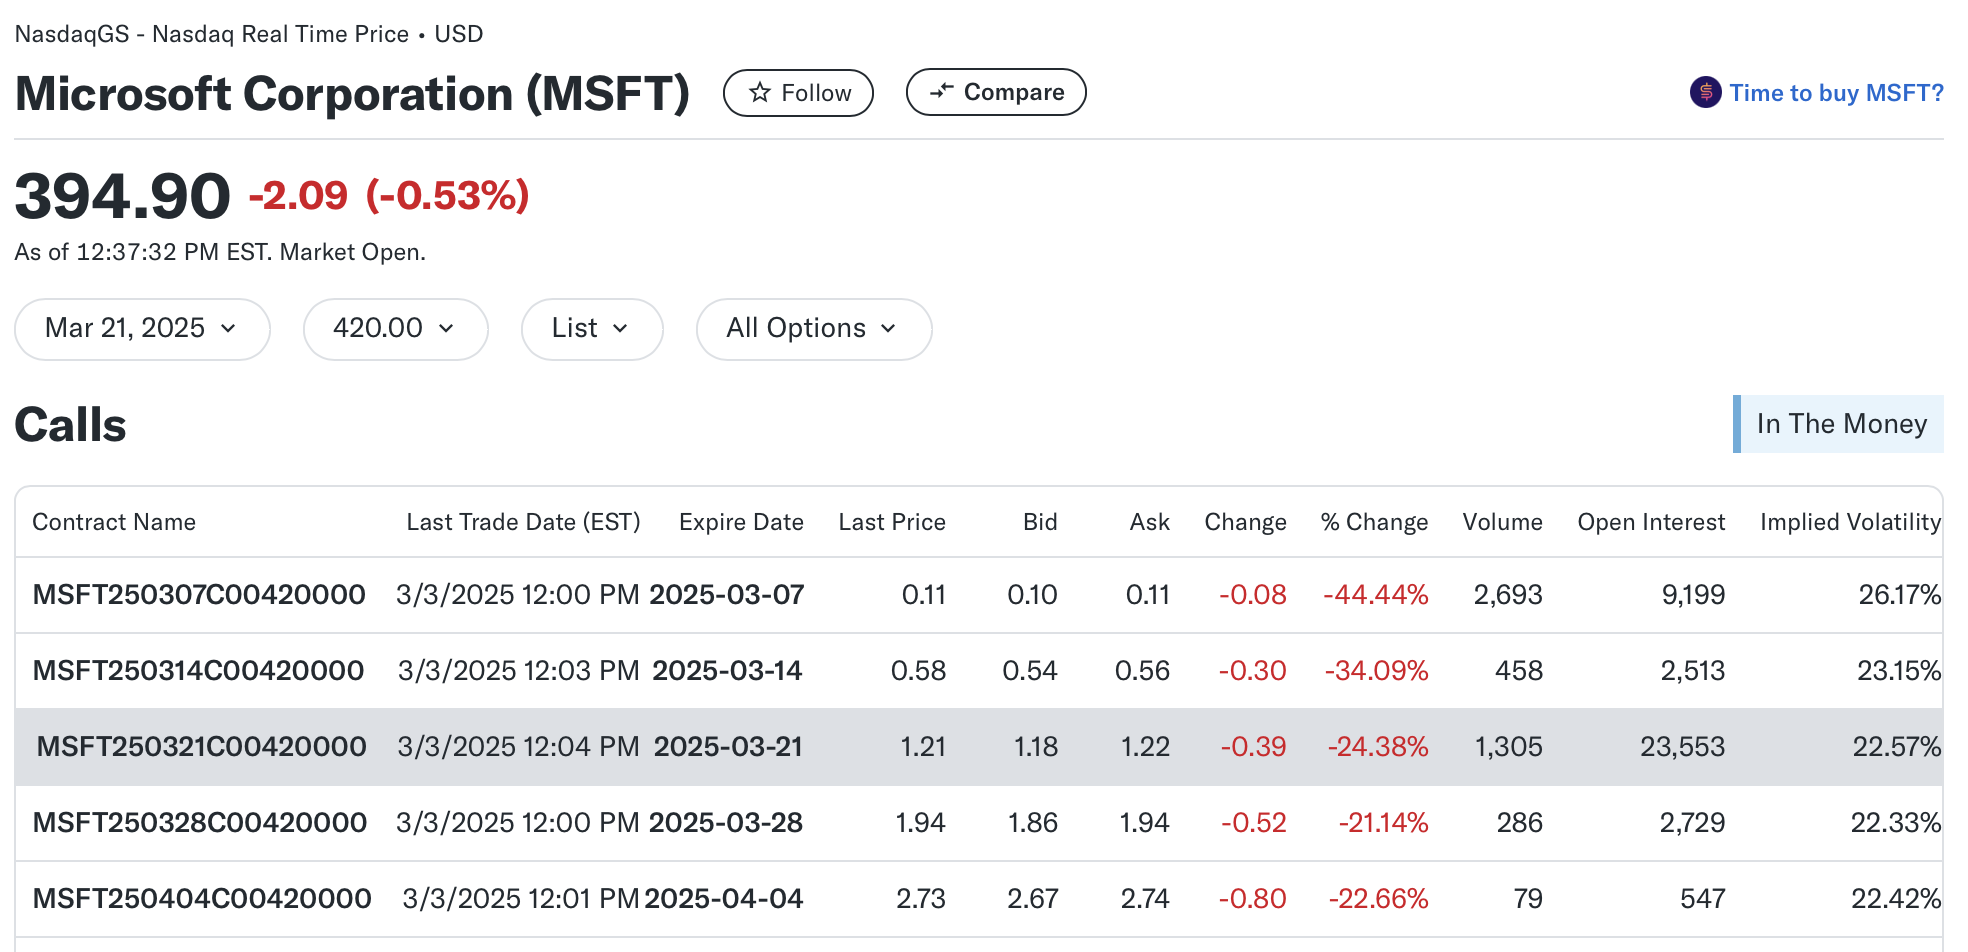
\includegraphics[width=0.9  \textwidth]{Q6_2}
	 \end{figure}
	 
	 
 
	 \clearpage
	 \subsection*{Question 7}
	 Download Excel options model with VBA code from the courseworks . Save as a source. Open in Excel. Modify the Black model for futures to Black-Scholes model for stocks paying dividends at rate q (like in the Hull’s book). Make the necessary changes in Visual Basic code. Use Excel help or consult TA’s if you do not know what to do. Check that code works and submit the code printout.
	 
	 \textbf{Answer}
	 
	 	\begin{figure}[h]
	 		\caption{The Printout of the B-S Model Re-implemented in Excel}
	 	\centering
	 	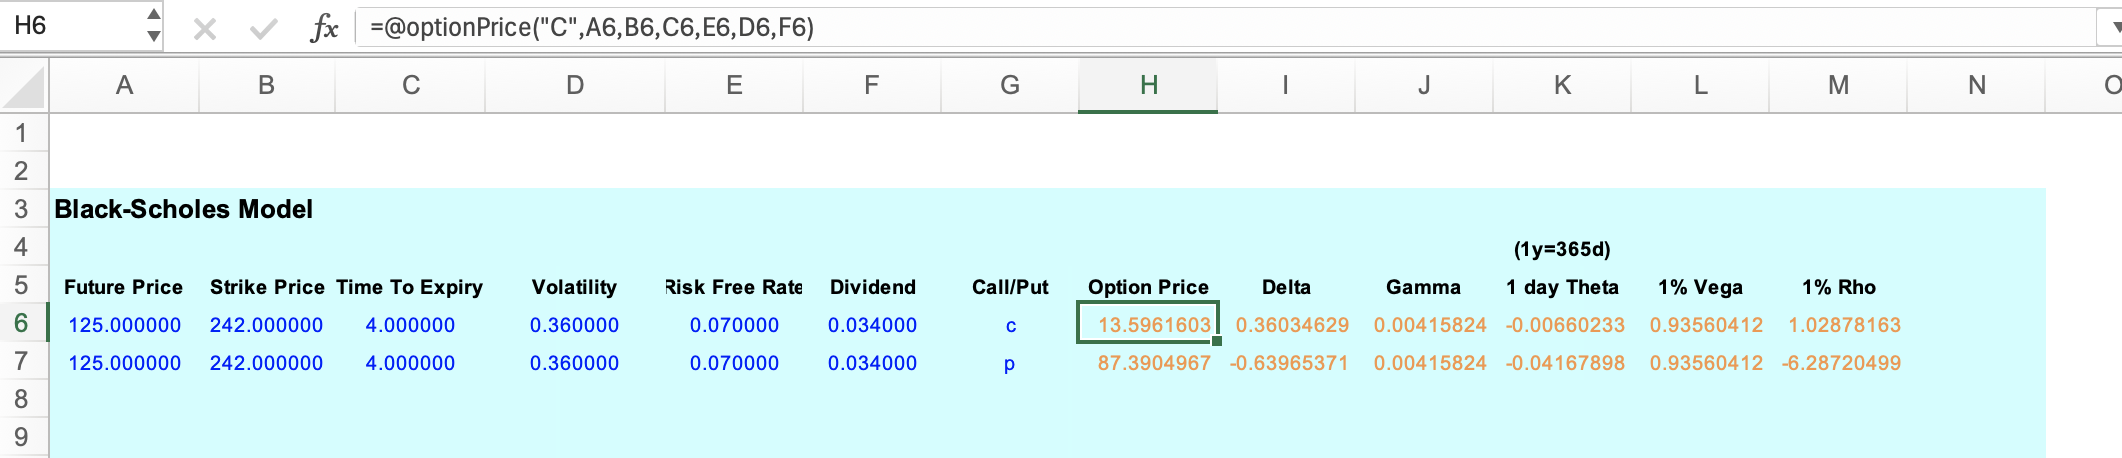
\includegraphics[width=1\textwidth]{Q7}
	 \end{figure}
 
  \begin{lstlisting}
     Function OptionPrice(OptionType As String, S As Double, X As Double, T As Double, r As Double, v As Double, d As Double) As Double
     dOne = (Log(S / X) + (r - d + 0.5 * v ^ 2) * T) / (v * (Sqr(T)))
     NdOne = Exp(-(dOne(S, X, T, r, v, d) ^ 2) / 2) / (Sqr(2 * 
     dTwo = dOne(S, X, T, r, v, d) - v * Sqr(T)
     NdTwo = Application.NormSDist(dTwo(S, X, T, r, v, d))
     If OptionType = "C" Then
     OptionPrice = Exp(-d * T) * S * Application.NormSDist(dOne(S, X, T, r, v, d)) - X * Exp(-r * T) * Application.NormSDist(dOne(S, X, T, r, v, d) - v * Sqr(T))
     ElseIf OptionType = "P" Then
     OptionPrice = X * Exp(-r * T) * Application.NormSDist(-dTwo(S, X, T, r, v, d)) - Exp(-d * T) * S * Application.NormSDist(-dOne(S, X, T, r, v, d))
     End If
     End Function
     
     Function OptionDelta(OptionType As String, S As Double, X As Double, T As Double, r As Double, v As Double, d As Double) As Double
     If OptionType = "C" Then
     OptionDelta = Application.NormSDist(dOne(S, X, T, r, v, d))
     ElseIf OptionType = "P" Then
     OptionDelta = Application.NormSDist(dOne(S, X, T, r, v, d)) - 1
     End If
     End Function
     
     Function OptionTheta(OptionType As String, S As Double, X As Double, T As Double, r As Double, v As Double, d As Double) As Double
     dOne = (Log(S / X) + (r - d + 0.5 * v ^ 2) * T) / (v * (Sqr(T)))
     NdOne = Exp(-(dOne(S, X, T, r, v, d) ^ 2) / 2) / (Sqr(2 * 
     dTwo = dOne(S, X, T, r, v, d) - v * Sqr(T)
     NdTwo = Application.NormSDist(dTwo(S, X, T, r, v, d))
     If OptionType = "C" Then
     OptionTheta = -((S * v * NdOne(S, X, T, r, v, d)) / (2 * Sqr(T)) - r * X * Exp(-r * (T)) * NdTwo(S, X, T, r, v, d)) / 365
     ElseIf OptionType = "P" Then
     OptionTheta = -((S * v * NdOne(S, X, T, r, v, d)) / (2 * Sqr(T)) + r * X * Exp(-r * (T)) * (1 - NdTwo(S, X, T, r, v, d))) / 365
     End If
     End Function
     
     Function Gamma(S As Double, X As Double, T As Double, r As Double, v As Double, d As Double) As Double
     Gamma = NdOne(S, X, T, r, v, d) / (S * (v * Sqr(T)))
     End Function
     
     Function Vega(S As Double, X As Double, T As Double, r As Double, v As Double, d As Double) As Double
     Vega = 0.01 * S * Sqr(T) * NdOne(S, X, T, r, v, d)
     End Function
     
     Function OptionRho(OptionType As String, S As Double, X As Double, T As Double, r As Double, v As Double, d As Double) As Double
     If OptionType = "C" Then
     OptionRho = 0.01 * X * T * Exp(-r * T) * Application.NormSDist(dTwo(S, X, T, r, v, d))
     ElseIf OptionType = "P" Then
     OptionRho = -0.01 * X * T * Exp(-r * T) * (1 - Application.NormSDist(dTwo(S, X, T, r, v, d)))
     End If
     End Function
\end{lstlisting}
	 
	 \subsection*{Question 8}
	 Download Excel Brownian Motion model from the courseworks. Save as a source. Open in Excel. Modify it to Geometric Brownian motion with growth rate $\mu$ = 0.04, volatility $\sigma$ = 0.20 and 250 trajectories. Submit excel formulas printout. Geometric Brownian motion starts with positive $X_0$ so you must change a starting value from 0 to a positive number that you may choose (you can choose 1, 100 or other positive number).
	 
	 
	 \textbf{Answer}
	 
	 The number for $X_0$ I chose was 20, I firstly put several parameters in the \texttt{A} column (for time step, it is 250).
	 
	 	\begin{figure}[h]
	 		\caption{Settings in my Excel}
	 	\centering
	 	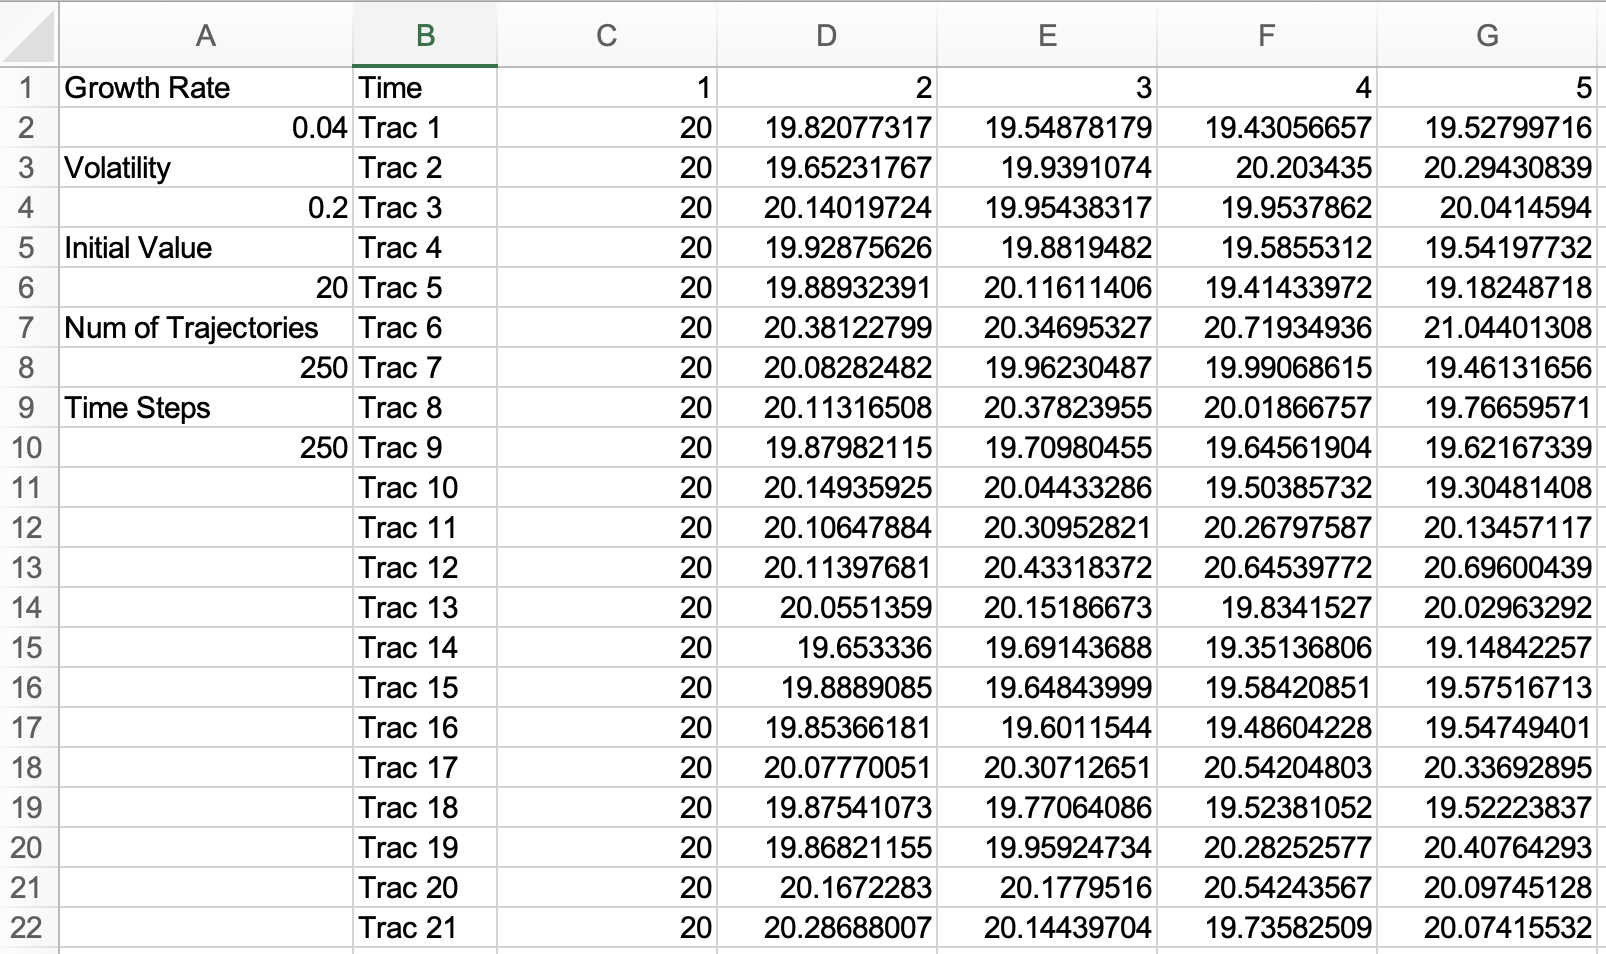
\includegraphics[width=0.7\textwidth]{Q8_1}
	 \end{figure}
	 
	  In \texttt{D2}, I set the formula to be \texttt{=C2*EXP((\$A\$2-0.5*\$A\$4\^{}2)*(1/250)+\$A\$4*SQRT(1/250)*NORMSINV(RAND()))}. The final printout is:
	 
	 \begin{figure}
	 	\caption{Geometric Brownian Motion with 250 Trajectories}
	 	\centering
	 	\includegraphics[width=1\textwidth]{Q8_2}
	 \end{figure}
 
 \clearpage
 
 Out of interest, I redid it in R:
 
 \begin{lstlisting}
     X0 <- 20
     mu <- 0.04
     sigma <- 0.20
     n <- 250
     T <- 1
     N <- 250
     dt <- T / N
     
     # Generate time vector
     time <- seq(0, T, by = dt)
     
     # Initialize matrix to store trajectories
     X <- matrix(NA, nrow = N + 1, ncol = n)
     X[1, ] <- X0
     
     # Simulate GBM
     set.seed(123)  # For reproducibility
     for (i in 1:n) {
     	for (j in 2:(N + 1)) {
     		dW <- rnorm(1, mean = 0, sd = sqrt(dt))
     		X[j, i] <- X[j - 1, i] * exp((mu - 0.5 * sigma^2) * dt + sigma * dW)
     	}
     }
     
     # Convert to data frame for plotting
     X_df <- as.data.frame(X)
     X_df$time <- time
     X_long <- melt(X_df, id.vars = "time", variable.name = "trajectory", value.name = "price")
     
     # Plot the trajectories
     ggplot(X_long, aes(x = time, y = price, group = trajectory)) +
     geom_line(alpha = 0.5) +
     labs(
     x = "Time",
     y = "Price") +
     theme_minimal()
 \end{lstlisting}

One interesting thing I noticed is that the set of trajectories tend to move upward, that's because there exists a drift term $\mu$, which is typically positive in financial implications (and also in this case). Thus we can notice as time goes on, the trajectories get out of 30 in both plots.

  \begin{figure}
 	\caption{Geometric Brownian Motion with 250 Trajectories Generated in R}
 	\centering
 	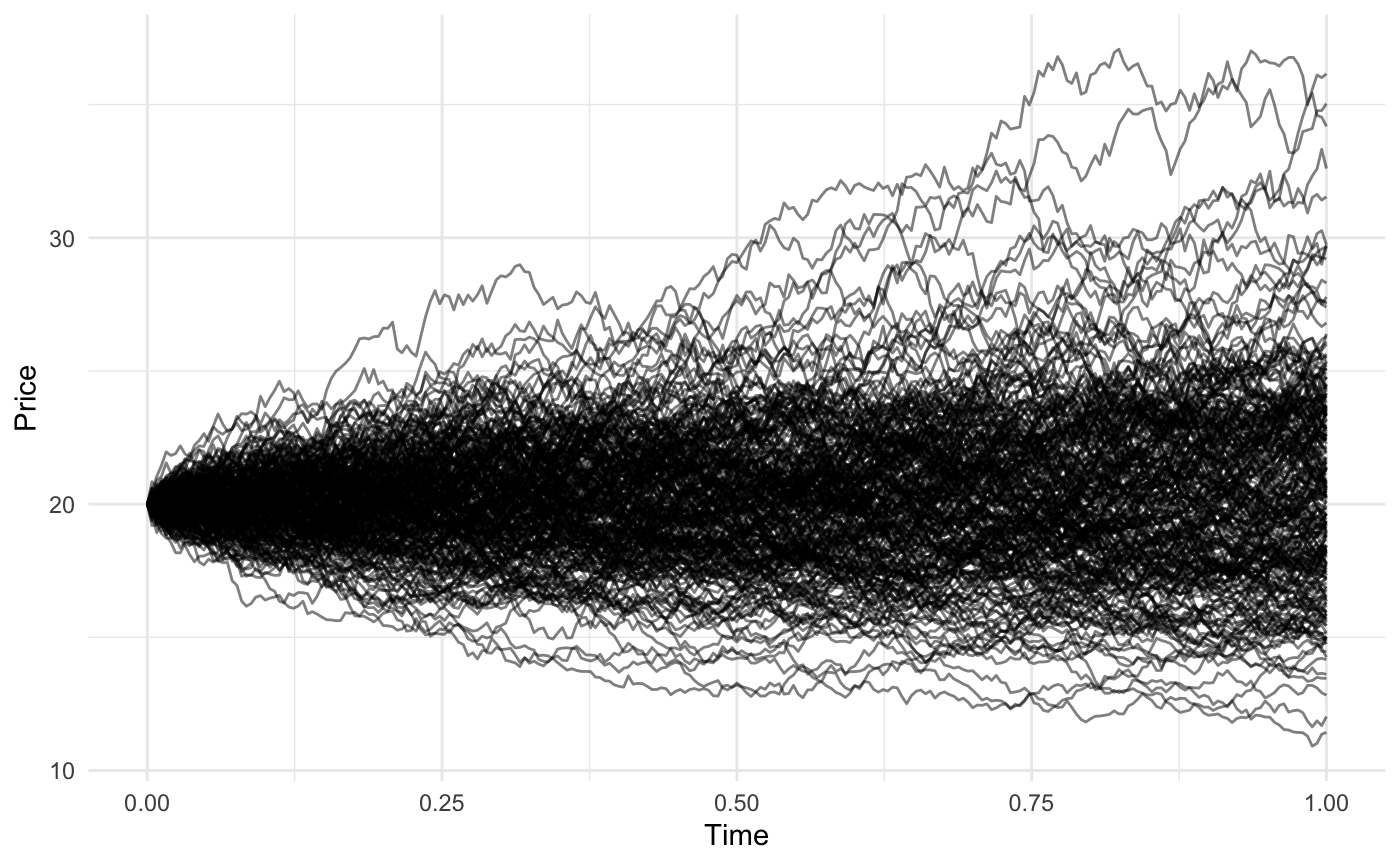
\includegraphics[width=1\textwidth]{Q8_3}
 \end{figure}
	 
	 
	\end{document}